\documentclass[twoside]{book}

% Packages required by doxygen
\usepackage{fixltx2e}
\usepackage{calc}
\usepackage{doxygen}
\usepackage[export]{adjustbox} % also loads graphicx
\usepackage{graphicx}
\usepackage[utf8]{inputenc}
\usepackage{makeidx}
\usepackage{multicol}
\usepackage{multirow}
\PassOptionsToPackage{warn}{textcomp}
\usepackage{textcomp}
\usepackage[nointegrals]{wasysym}
\usepackage[table]{xcolor}

% Font selection
\usepackage[T1]{fontenc}
\usepackage[scaled=.90]{helvet}
\usepackage{courier}
\usepackage{amssymb}
\usepackage{sectsty}
\renewcommand{\familydefault}{\sfdefault}
\allsectionsfont{%
  \fontseries{bc}\selectfont%
  \color{darkgray}%
}
\renewcommand{\DoxyLabelFont}{%
  \fontseries{bc}\selectfont%
  \color{darkgray}%
}
\newcommand{\+}{\discretionary{\mbox{\scriptsize$\hookleftarrow$}}{}{}}

% Page & text layout
\usepackage{geometry}
\geometry{%
  a4paper,%
  top=2.5cm,%
  bottom=2.5cm,%
  left=2.5cm,%
  right=2.5cm%
}
\tolerance=750
\hfuzz=15pt
\hbadness=750
\setlength{\emergencystretch}{15pt}
\setlength{\parindent}{0cm}
\setlength{\parskip}{0.2cm}
\makeatletter
\renewcommand{\paragraph}{%
  \@startsection{paragraph}{4}{0ex}{-1.0ex}{1.0ex}{%
    \normalfont\normalsize\bfseries\SS@parafont%
  }%
}
\renewcommand{\subparagraph}{%
  \@startsection{subparagraph}{5}{0ex}{-1.0ex}{1.0ex}{%
    \normalfont\normalsize\bfseries\SS@subparafont%
  }%
}
\makeatother

% Headers & footers
\usepackage{fancyhdr}
\pagestyle{fancyplain}
\fancyhead[LE]{\fancyplain{}{\bfseries\thepage}}
\fancyhead[CE]{\fancyplain{}{}}
\fancyhead[RE]{\fancyplain{}{\bfseries\leftmark}}
\fancyhead[LO]{\fancyplain{}{\bfseries\rightmark}}
\fancyhead[CO]{\fancyplain{}{}}
\fancyhead[RO]{\fancyplain{}{\bfseries\thepage}}
\fancyfoot[LE]{\fancyplain{}{}}
\fancyfoot[CE]{\fancyplain{}{}}
\fancyfoot[RE]{\fancyplain{}{\bfseries\scriptsize Generated on Sat Feb 18 2017 19\+:10\+:03 for My Project by Doxygen }}
\fancyfoot[LO]{\fancyplain{}{\bfseries\scriptsize Generated on Sat Feb 18 2017 19\+:10\+:03 for My Project by Doxygen }}
\fancyfoot[CO]{\fancyplain{}{}}
\fancyfoot[RO]{\fancyplain{}{}}
\renewcommand{\footrulewidth}{0.4pt}
\renewcommand{\chaptermark}[1]{%
  \markboth{#1}{}%
}
\renewcommand{\sectionmark}[1]{%
  \markright{\thesection\ #1}%
}

% Indices & bibliography
\usepackage{natbib}
\usepackage[titles]{tocloft}
\setcounter{tocdepth}{3}
\setcounter{secnumdepth}{5}
\makeindex

% Hyperlinks (required, but should be loaded last)
\usepackage{ifpdf}
\ifpdf
  \usepackage[pdftex,pagebackref=true]{hyperref}
\else
  \usepackage[ps2pdf,pagebackref=true]{hyperref}
\fi
\hypersetup{%
  colorlinks=true,%
  linkcolor=blue,%
  citecolor=blue,%
  unicode%
}

% Custom commands
\newcommand{\clearemptydoublepage}{%
  \newpage{\pagestyle{empty}\cleardoublepage}%
}


%===== C O N T E N T S =====

\begin{document}

% Titlepage & ToC
\hypersetup{pageanchor=false,
             bookmarks=true,
             bookmarksnumbered=true,
             pdfencoding=unicode
            }
\pagenumbering{roman}
\begin{titlepage}
\vspace*{7cm}
\begin{center}%
{\Large My Project }\\
\vspace*{1cm}
{\large Generated by Doxygen 1.8.9.1}\\
\vspace*{0.5cm}
{\small Sat Feb 18 2017 19:10:03}\\
\end{center}
\end{titlepage}
\clearemptydoublepage
\tableofcontents
\clearemptydoublepage
\pagenumbering{arabic}
\hypersetup{pageanchor=true}

%--- Begin generated contents ---
\chapter{Hierarchical Index}
\section{Class Hierarchy}
This inheritance list is sorted roughly, but not completely, alphabetically\+:\begin{DoxyCompactList}
\item J\+Frame\begin{DoxyCompactList}
\item \contentsline{section}{Main\+Frame\+Part1}{\pageref{classMainFramePart1}}{}
\item \contentsline{section}{Main\+Frame\+Part2}{\pageref{classMainFramePart2}}{}
\item \contentsline{section}{Remote\+Control}{\pageref{classRemoteControl}}{}
\end{DoxyCompactList}
\item \contentsline{section}{Remote\+Client}{\pageref{classRemoteClient}}{}
\end{DoxyCompactList}

\chapter{Class Index}
\section{Class List}
Here are the classes, structs, unions and interfaces with brief descriptions\+:\begin{DoxyCompactList}
\item\contentsline{section}{\hyperlink{structcppu_1_1TCPServer_1_1Callback}{cppu\+::\+T\+C\+P\+Server\+::\+Callback} \\*\hyperlink{structcppu_1_1TCPServer_1_1Callback}{Callback} interface }{\pageref{structcppu_1_1TCPServer_1_1Callback}}{}
\item\contentsline{section}{\hyperlink{structcppu_1_1TCPServer_1_1CallbackMethod}{cppu\+::\+T\+C\+P\+Server\+::\+Callback\+Method$<$ T $>$} }{\pageref{structcppu_1_1TCPServer_1_1CallbackMethod}}{}
\item\contentsline{section}{\hyperlink{classData}{Data} \\*\hyperlink{classData}{Data} class. This is the class which is used to keep tracks of all the multimediaobjects and groups created. \hyperlink{classData}{Data} is stored using std\+::map, using names as keys. We use smart pointers everywhere for a better memory usage }{\pageref{classData}}{}
\item\contentsline{section}{\hyperlink{classFilm}{Film} \\*\hyperlink{classFilm}{Film} class, extends the video class. Using pointers for learning purpose }{\pageref{classFilm}}{}
\item\contentsline{section}{\hyperlink{classGroup}{Group} \\*\hyperlink{classGroup}{Group} class extends the std\+::list class. We store shared\+\_\+ptr of multimedia objects to prevent any memory leak }{\pageref{classGroup}}{}
\item\contentsline{section}{\hyperlink{structcppu_1_1InputBuffer}{cppu\+::\+Input\+Buffer} }{\pageref{structcppu_1_1InputBuffer}}{}
\item\contentsline{section}{\hyperlink{classMultimediaObject}{Multimedia\+Object} \\*Abstract class for a multimedia object }{\pageref{classMultimediaObject}}{}
\item\contentsline{section}{\hyperlink{classPicture}{Picture} \\*\hyperlink{classPicture}{Picture} class, extends the abstract class \hyperlink{classMultimediaObject}{Multimedia\+Object} }{\pageref{classPicture}}{}
\item\contentsline{section}{\hyperlink{classcppu_1_1ServerSocket}{cppu\+::\+Server\+Socket} \\*T\+C\+P/\+I\+P server socket. This class implements a T\+C\+P/\+I\+P socket that waits for requests to come in over the network. A\+F\+\_\+\+I\+N\+E\+T connections following the I\+Pv4 Internet protocol are supported }{\pageref{classcppu_1_1ServerSocket}}{}
\item\contentsline{section}{\hyperlink{classcppu_1_1Socket}{cppu\+::\+Socket} \\*T\+C\+P/\+I\+P or U\+D\+P/\+Datagram socket. This class encapsulates a T\+C\+P/\+I\+P or U\+D\+P/\+Datagram socket. A\+F\+\_\+\+I\+N\+E\+T connections following the I\+Pv4 Internet protocol are supported }{\pageref{classcppu_1_1Socket}}{}
\item\contentsline{section}{\hyperlink{classcppu_1_1SocketBuffer}{cppu\+::\+Socket\+Buffer} \\*Preserves record boundaries when exchanging data between connected T\+C\+P/\+I\+P sockets. This class ensures that one call to \hyperlink{classcppu_1_1SocketBuffer_a92ae0351aaee8719d34e8c4618495d59}{write\+Line()} corresponds to one and exactly one call to \hyperlink{classcppu_1_1SocketBuffer_a222769d3776b9cbd3a727ee1f0e60358}{read\+Line()} on the other side. This differs from the behavior of \hyperlink{classcppu_1_1Socket_aeac77f859159715e2d63a5a0dc118788}{Socket\+::send()} and \hyperlink{classcppu_1_1Socket_a37c382af52cc02f92c0e19a0c6e0e04f}{Socket\+::receive()} because T\+C\+P/\+I\+P connected sockets do not preserve record boundaries. \hyperlink{classcppu_1_1SocketBuffer_a92ae0351aaee8719d34e8c4618495d59}{write\+Line()} and \hyperlink{classcppu_1_1SocketBuffer_a222769d3776b9cbd3a727ee1f0e60358}{read\+Line()} solve this problem by automatically adding and searching for a separator between successive lines }{\pageref{classcppu_1_1SocketBuffer}}{}
\item\contentsline{section}{\hyperlink{classcppu_1_1TCPConnection}{cppu\+::\+T\+C\+P\+Connection} \\*Connection with a given client. Each \hyperlink{classcppu_1_1TCPConnection}{T\+C\+P\+Connection} uses a different thread }{\pageref{classcppu_1_1TCPConnection}}{}
\item\contentsline{section}{\hyperlink{classcppu_1_1TCPLock}{cppu\+::\+T\+C\+P\+Lock} \\*Locks the server in read mode or in write mode. Must be created {\itshape in the stack} by the callback method }{\pageref{classcppu_1_1TCPLock}}{}
\item\contentsline{section}{\hyperlink{classcppu_1_1TCPServer}{cppu\+::\+T\+C\+P\+Server} \\*T\+C\+P/\+I\+P I\+Pv4 server. The server supports T\+C\+P/\+I\+P A\+F\+\_\+\+I\+N\+E\+T connections (following the I\+Pv4 Internet protocol) with multiple clients. One thread is used per client }{\pageref{classcppu_1_1TCPServer}}{}
\item\contentsline{section}{\hyperlink{classVideo}{Video} \\*\hyperlink{classVideo}{Video} class, extends the abstract class \hyperlink{classMultimediaObject}{Multimedia\+Object} }{\pageref{classVideo}}{}
\end{DoxyCompactList}

\chapter{Class Documentation}
\hypertarget{structcppu_1_1TCPServer_1_1Callback}{}\section{cppu\+:\+:T\+C\+P\+Server\+:\+:Callback Struct Reference}
\label{structcppu_1_1TCPServer_1_1Callback}\index{cppu\+::\+T\+C\+P\+Server\+::\+Callback@{cppu\+::\+T\+C\+P\+Server\+::\+Callback}}


\hyperlink{structcppu_1_1TCPServer_1_1Callback}{Callback} interface.  




{\ttfamily \#include $<$tcp\+Server.\+h$>$}



Inheritance diagram for cppu\+:\+:T\+C\+P\+Server\+:\+:Callback\+:
\nopagebreak
\begin{figure}[H]
\begin{center}
\leavevmode
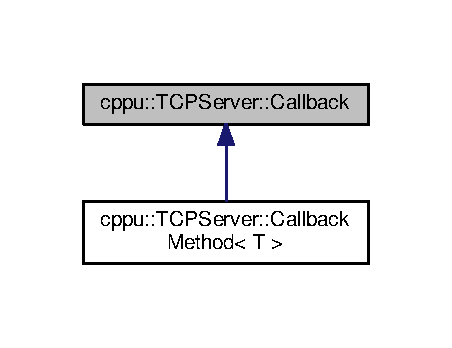
\includegraphics[width=217pt]{structcppu_1_1TCPServer_1_1Callback__inherit__graph}
\end{center}
\end{figure}
\subsection*{Public Member Functions}
\begin{DoxyCompactItemize}
\item 
\hypertarget{structcppu_1_1TCPServer_1_1Callback_aabe4b0b30e14ddeb7c0c02aa3a335eba}{}virtual bool {\bfseries call} (\hyperlink{classcppu_1_1TCPConnection}{T\+C\+P\+Connection} \&cnx, const std\+::string \&request, std\+::string \&response)=0\label{structcppu_1_1TCPServer_1_1Callback_aabe4b0b30e14ddeb7c0c02aa3a335eba}

\end{DoxyCompactItemize}


\subsection{Detailed Description}
\hyperlink{structcppu_1_1TCPServer_1_1Callback}{Callback} interface. 

The documentation for this struct was generated from the following file\+:\begin{DoxyCompactItemize}
\item 
tcp\+Server.\+h\end{DoxyCompactItemize}

\hypertarget{structcppu_1_1TCPServer_1_1CallbackMethod}{}\section{cppu\+:\+:T\+C\+P\+Server\+:\+:Callback\+Method$<$ T $>$ Struct Template Reference}
\label{structcppu_1_1TCPServer_1_1CallbackMethod}\index{cppu\+::\+T\+C\+P\+Server\+::\+Callback\+Method$<$ T $>$@{cppu\+::\+T\+C\+P\+Server\+::\+Callback\+Method$<$ T $>$}}


Inheritance diagram for cppu\+:\+:T\+C\+P\+Server\+:\+:Callback\+Method$<$ T $>$\+:
\nopagebreak
\begin{figure}[H]
\begin{center}
\leavevmode
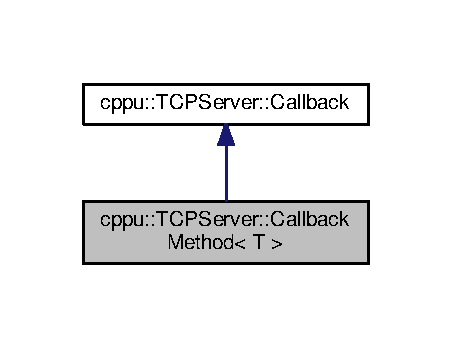
\includegraphics[width=217pt]{structcppu_1_1TCPServer_1_1CallbackMethod__inherit__graph}
\end{center}
\end{figure}


Collaboration diagram for cppu\+:\+:T\+C\+P\+Server\+:\+:Callback\+Method$<$ T $>$\+:
\nopagebreak
\begin{figure}[H]
\begin{center}
\leavevmode
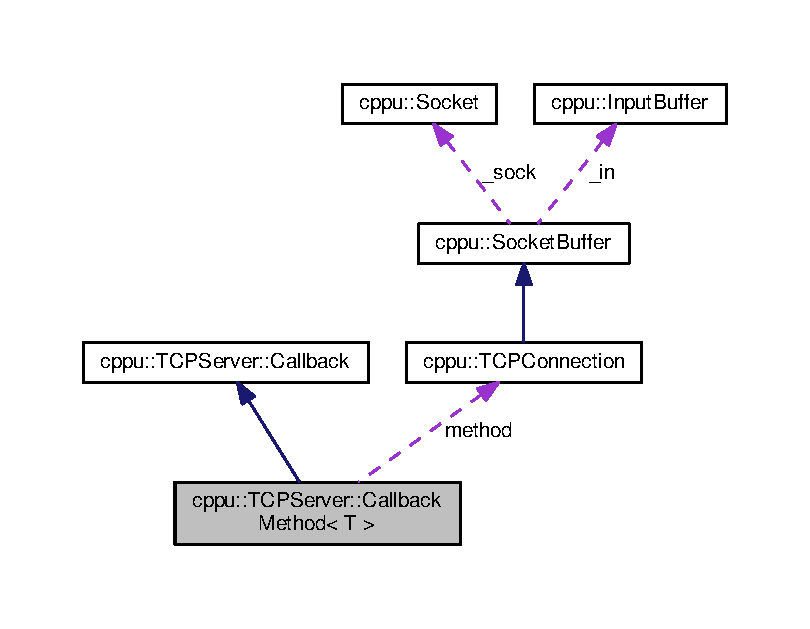
\includegraphics[width=350pt]{structcppu_1_1TCPServer_1_1CallbackMethod__coll__graph}
\end{center}
\end{figure}
\subsection*{Public Types}
\begin{DoxyCompactItemize}
\item 
\hypertarget{structcppu_1_1TCPServer_1_1CallbackMethod_a6f71d878bd072aadf40d96d1db18eecd}{}typedef bool(T\+::$\ast$ {\bfseries Fun}) (\hyperlink{classcppu_1_1TCPConnection}{T\+C\+P\+Connection} \&, const std\+::string \&, std\+::string \&)\label{structcppu_1_1TCPServer_1_1CallbackMethod_a6f71d878bd072aadf40d96d1db18eecd}

\end{DoxyCompactItemize}
\subsection*{Public Member Functions}
\begin{DoxyCompactItemize}
\item 
\hypertarget{structcppu_1_1TCPServer_1_1CallbackMethod_a0c6ceee6db8c67ef56fb26d1df52140f}{}{\bfseries Callback\+Method} (T \&obj, Fun method)\label{structcppu_1_1TCPServer_1_1CallbackMethod_a0c6ceee6db8c67ef56fb26d1df52140f}

\item 
\hypertarget{structcppu_1_1TCPServer_1_1CallbackMethod_a0c11039d0ed983c03a614d0764df3793}{}virtual bool {\bfseries call} (\hyperlink{classcppu_1_1TCPConnection}{T\+C\+P\+Connection} \&cnx, const std\+::string \&req, std\+::string \&resp)\label{structcppu_1_1TCPServer_1_1CallbackMethod_a0c11039d0ed983c03a614d0764df3793}

\end{DoxyCompactItemize}
\subsection*{Public Attributes}
\begin{DoxyCompactItemize}
\item 
\hypertarget{structcppu_1_1TCPServer_1_1CallbackMethod_ae480535d346efc119fb5c43880f349c8}{}T \& {\bfseries obj}\label{structcppu_1_1TCPServer_1_1CallbackMethod_ae480535d346efc119fb5c43880f349c8}

\item 
\hypertarget{structcppu_1_1TCPServer_1_1CallbackMethod_aab858a039ddee71fb65a0e35c173f067}{}Fun {\bfseries method}\label{structcppu_1_1TCPServer_1_1CallbackMethod_aab858a039ddee71fb65a0e35c173f067}

\end{DoxyCompactItemize}


The documentation for this struct was generated from the following file\+:\begin{DoxyCompactItemize}
\item 
tcp\+Server.\+h\end{DoxyCompactItemize}

\hypertarget{classData}{}\section{Data Class Reference}
\label{classData}\index{Data@{Data}}


\hyperlink{classData}{Data} class. This is the class which is used to keep tracks of all the multimediaobjects and groups created. \hyperlink{classData}{Data} is stored using std\+::map, using names as keys. We use smart pointers everywhere for a better memory usage.  




{\ttfamily \#include $<$Data.\+h$>$}

\subsection*{Public Member Functions}
\begin{DoxyCompactItemize}
\item 
virtual \hyperlink{classData_aab31956423290f0d62dcca47ab4d16dd}{$\sim$\+Data} ()
\begin{DoxyCompactList}\small\item\em Destroys the data object. \end{DoxyCompactList}\item 
\hypertarget{classData_af11f741cb7f587e2e495452a8905a22a}{}\hyperlink{classData_af11f741cb7f587e2e495452a8905a22a}{Data} ()\label{classData_af11f741cb7f587e2e495452a8905a22a}

\begin{DoxyCompactList}\small\item\em Creates the data object. \end{DoxyCompactList}\item 
Video\+Ptr \hyperlink{classData_a9a86e93e191dc4244c18928b908861cc}{new\+Video} (const string \&name)
\begin{DoxyCompactList}\small\item\em Used to create a new blank video. \end{DoxyCompactList}\item 
Video\+Ptr \hyperlink{classData_a9e7919b3ca3390c0002cd2ba2854bbc4}{new\+Video} (istream \&is)
\begin{DoxyCompactList}\small\item\em Used to create a new video from a file. \end{DoxyCompactList}\item 
Pic\+Ptr \hyperlink{classData_a1fb51b0d2aee38a233b505c8e4fb862d}{new\+Picture} (const string \&name)
\begin{DoxyCompactList}\small\item\em Used to create a new blank picture. \end{DoxyCompactList}\item 
Pic\+Ptr \hyperlink{classData_ac0d33face47c9aa31c5ced3bba1ba348}{new\+Picture} (istream \&is)
\begin{DoxyCompactList}\small\item\em Used to create a new picture from a file. \end{DoxyCompactList}\item 
Film\+Ptr \hyperlink{classData_abf84f4ca94b966ffe9f0a5272e4048d7}{new\+Film} (const string \&name)
\begin{DoxyCompactList}\small\item\em Used to create a new blank film. \end{DoxyCompactList}\item 
Film\+Ptr \hyperlink{classData_aa14f12c39b4d568353606420b691296f}{new\+Film} (istream \&is)
\begin{DoxyCompactList}\small\item\em Used to create a new film from a file. \end{DoxyCompactList}\item 
Group\+Ptr \hyperlink{classData_a94d766d884a27444fdca887a60e1162c}{new\+Group} (const string \&name)
\begin{DoxyCompactList}\small\item\em Used to create a new blank group. \end{DoxyCompactList}\item 
void \hyperlink{classData_a792f2e1f05c9d068892aad4940e27ff6}{display\+Elements} (ostream \&os) const 
\begin{DoxyCompactList}\small\item\em Displays info on all the elements of the m\+O\+Table. \end{DoxyCompactList}\item 
void \hyperlink{classData_ada79ae2968738413d48250a684ae63ec}{search\+Multimedia\+Object} (const string \&name, ostream \&os) const 
\begin{DoxyCompactList}\small\item\em Look for a multimedia object with the given name in the multimediaobject table. \end{DoxyCompactList}\item 
void \hyperlink{classData_ae4df938ba31a8359006e824a880559b3}{search\+Group} (const string \&name, ostream \&os) const 
\begin{DoxyCompactList}\small\item\em Look for a group with the given name in the group table. \end{DoxyCompactList}\item 
void \hyperlink{classData_a627fcf83d707dd0cef70245fe7785f4f}{play\+Multimedia\+Object} (const string \&name, ostream \&os) const 
\begin{DoxyCompactList}\small\item\em Play the multimedia object with the given name, displays error if we can\textquotesingle{}t find the object. \end{DoxyCompactList}\item 
bool \hyperlink{classData_a1e03c91a77ed0555dae82727dfcc8df9}{process\+Request} (\hyperlink{classcppu_1_1TCPConnection}{T\+C\+P\+Connection} \&cnx, const string \&request, string \&response)
\begin{DoxyCompactList}\small\item\em Process the request received from the server and sends back the appropriate answer. \end{DoxyCompactList}\item 
bool \hyperlink{classData_a72951a7406a853d0c05c5b02ca31eba2}{save} (const string \&file\+Name) const 
\begin{DoxyCompactList}\small\item\em Saves all data in the multimediaobject table. \end{DoxyCompactList}\item 
bool \hyperlink{classData_a1f31af0bd1cde50acd39b811245fe2c8}{load} (const string \&file\+Name)
\begin{DoxyCompactList}\small\item\em Loads data from the file in the multimedia object table. \end{DoxyCompactList}\end{DoxyCompactItemize}


\subsection{Detailed Description}
\hyperlink{classData}{Data} class. This is the class which is used to keep tracks of all the multimediaobjects and groups created. \hyperlink{classData}{Data} is stored using std\+::map, using names as keys. We use smart pointers everywhere for a better memory usage. 

\subsection{Constructor \& Destructor Documentation}
\hypertarget{classData_aab31956423290f0d62dcca47ab4d16dd}{}\index{Data@{Data}!````~Data@{$\sim$\+Data}}
\index{````~Data@{$\sim$\+Data}!Data@{Data}}
\subsubsection[{$\sim$\+Data}]{\setlength{\rightskip}{0pt plus 5cm}Data\+::$\sim$\+Data (
\begin{DoxyParamCaption}
{}
\end{DoxyParamCaption}
)\hspace{0.3cm}{\ttfamily [virtual]}}\label{classData_aab31956423290f0d62dcca47ab4d16dd}


Destroys the data object. 

No need to do anything in destructor thanks to smartpointers ! 

\subsection{Member Function Documentation}
\hypertarget{classData_a792f2e1f05c9d068892aad4940e27ff6}{}\index{Data@{Data}!display\+Elements@{display\+Elements}}
\index{display\+Elements@{display\+Elements}!Data@{Data}}
\subsubsection[{display\+Elements}]{\setlength{\rightskip}{0pt plus 5cm}void Data\+::display\+Elements (
\begin{DoxyParamCaption}
\item[{ostream \&}]{os}
\end{DoxyParamCaption}
) const}\label{classData_a792f2e1f05c9d068892aad4940e27ff6}


Displays info on all the elements of the m\+O\+Table. 


\begin{DoxyParams}{Parameters}
{\em os} & The output stream. \\
\hline
\end{DoxyParams}
\hypertarget{classData_a1f31af0bd1cde50acd39b811245fe2c8}{}\index{Data@{Data}!load@{load}}
\index{load@{load}!Data@{Data}}
\subsubsection[{load}]{\setlength{\rightskip}{0pt plus 5cm}bool Data\+::load (
\begin{DoxyParamCaption}
\item[{const string \&}]{file\+Name}
\end{DoxyParamCaption}
)}\label{classData_a1f31af0bd1cde50acd39b811245fe2c8}


Loads data from the file in the multimedia object table. 


\begin{DoxyParams}[1]{Parameters}
\mbox{\tt in}  & {\em file\+Name} & The file name from where we read the data.\\
\hline
\end{DoxyParams}
\begin{DoxyReturn}{Returns}
Returns true if successful, false otherwise. 
\end{DoxyReturn}
Opening file \hypertarget{classData_abf84f4ca94b966ffe9f0a5272e4048d7}{}\index{Data@{Data}!new\+Film@{new\+Film}}
\index{new\+Film@{new\+Film}!Data@{Data}}
\subsubsection[{new\+Film}]{\setlength{\rightskip}{0pt plus 5cm}Film\+Ptr Data\+::new\+Film (
\begin{DoxyParamCaption}
\item[{const string \&}]{name}
\end{DoxyParamCaption}
)}\label{classData_abf84f4ca94b966ffe9f0a5272e4048d7}


Used to create a new blank film. 


\begin{DoxyParams}[1]{Parameters}
\mbox{\tt in}  & {\em name} & The name\\
\hline
\end{DoxyParams}
\begin{DoxyReturn}{Returns}
Smart pointer to the film created. 
\end{DoxyReturn}
\hypertarget{classData_aa14f12c39b4d568353606420b691296f}{}\index{Data@{Data}!new\+Film@{new\+Film}}
\index{new\+Film@{new\+Film}!Data@{Data}}
\subsubsection[{new\+Film}]{\setlength{\rightskip}{0pt plus 5cm}Film\+Ptr Data\+::new\+Film (
\begin{DoxyParamCaption}
\item[{istream \&}]{is}
\end{DoxyParamCaption}
)}\label{classData_aa14f12c39b4d568353606420b691296f}


Used to create a new film from a file. 


\begin{DoxyParams}{Parameters}
{\em is} & input stream.\\
\hline
\end{DoxyParams}
\begin{DoxyReturn}{Returns}
Smart pointer to the film created. 
\end{DoxyReturn}
We read the data from the input stream \hypertarget{classData_a94d766d884a27444fdca887a60e1162c}{}\index{Data@{Data}!new\+Group@{new\+Group}}
\index{new\+Group@{new\+Group}!Data@{Data}}
\subsubsection[{new\+Group}]{\setlength{\rightskip}{0pt plus 5cm}Group\+Ptr Data\+::new\+Group (
\begin{DoxyParamCaption}
\item[{const string \&}]{name}
\end{DoxyParamCaption}
)}\label{classData_a94d766d884a27444fdca887a60e1162c}


Used to create a new blank group. 


\begin{DoxyParams}[1]{Parameters}
\mbox{\tt in}  & {\em name} & The name\\
\hline
\end{DoxyParams}
\begin{DoxyReturn}{Returns}
Smart pointer to the group created. 
\end{DoxyReturn}
\hypertarget{classData_a1fb51b0d2aee38a233b505c8e4fb862d}{}\index{Data@{Data}!new\+Picture@{new\+Picture}}
\index{new\+Picture@{new\+Picture}!Data@{Data}}
\subsubsection[{new\+Picture}]{\setlength{\rightskip}{0pt plus 5cm}Pic\+Ptr Data\+::new\+Picture (
\begin{DoxyParamCaption}
\item[{const string \&}]{name}
\end{DoxyParamCaption}
)}\label{classData_a1fb51b0d2aee38a233b505c8e4fb862d}


Used to create a new blank picture. 


\begin{DoxyParams}[1]{Parameters}
\mbox{\tt in}  & {\em name} & The name\\
\hline
\end{DoxyParams}
\begin{DoxyReturn}{Returns}
Smart pointer to the picture created. 
\end{DoxyReturn}
\hypertarget{classData_ac0d33face47c9aa31c5ced3bba1ba348}{}\index{Data@{Data}!new\+Picture@{new\+Picture}}
\index{new\+Picture@{new\+Picture}!Data@{Data}}
\subsubsection[{new\+Picture}]{\setlength{\rightskip}{0pt plus 5cm}Pic\+Ptr Data\+::new\+Picture (
\begin{DoxyParamCaption}
\item[{istream \&}]{is}
\end{DoxyParamCaption}
)}\label{classData_ac0d33face47c9aa31c5ced3bba1ba348}


Used to create a new picture from a file. 


\begin{DoxyParams}{Parameters}
{\em is} & input stream.\\
\hline
\end{DoxyParams}
\begin{DoxyReturn}{Returns}
Smart pointer to the picture created. 
\end{DoxyReturn}
We read the data from the input stream \hypertarget{classData_a9a86e93e191dc4244c18928b908861cc}{}\index{Data@{Data}!new\+Video@{new\+Video}}
\index{new\+Video@{new\+Video}!Data@{Data}}
\subsubsection[{new\+Video}]{\setlength{\rightskip}{0pt plus 5cm}Video\+Ptr Data\+::new\+Video (
\begin{DoxyParamCaption}
\item[{const string \&}]{name}
\end{DoxyParamCaption}
)}\label{classData_a9a86e93e191dc4244c18928b908861cc}


Used to create a new blank video. 


\begin{DoxyParams}[1]{Parameters}
\mbox{\tt in}  & {\em name} & The name\\
\hline
\end{DoxyParams}
\begin{DoxyReturn}{Returns}
Smart pointer to the video created. 
\end{DoxyReturn}
\hypertarget{classData_a9e7919b3ca3390c0002cd2ba2854bbc4}{}\index{Data@{Data}!new\+Video@{new\+Video}}
\index{new\+Video@{new\+Video}!Data@{Data}}
\subsubsection[{new\+Video}]{\setlength{\rightskip}{0pt plus 5cm}Video\+Ptr Data\+::new\+Video (
\begin{DoxyParamCaption}
\item[{istream \&}]{is}
\end{DoxyParamCaption}
)}\label{classData_a9e7919b3ca3390c0002cd2ba2854bbc4}


Used to create a new video from a file. 


\begin{DoxyParams}{Parameters}
{\em is} & input stream.\\
\hline
\end{DoxyParams}
\begin{DoxyReturn}{Returns}
Smart pointer to the video created. 
\end{DoxyReturn}
We read the data from the input stream \hypertarget{classData_a627fcf83d707dd0cef70245fe7785f4f}{}\index{Data@{Data}!play\+Multimedia\+Object@{play\+Multimedia\+Object}}
\index{play\+Multimedia\+Object@{play\+Multimedia\+Object}!Data@{Data}}
\subsubsection[{play\+Multimedia\+Object}]{\setlength{\rightskip}{0pt plus 5cm}void Data\+::play\+Multimedia\+Object (
\begin{DoxyParamCaption}
\item[{const string \&}]{name, }
\item[{ostream \&}]{os}
\end{DoxyParamCaption}
) const}\label{classData_a627fcf83d707dd0cef70245fe7785f4f}


Play the multimedia object with the given name, displays error if we can\textquotesingle{}t find the object. 


\begin{DoxyParams}[1]{Parameters}
\mbox{\tt in}  & {\em name} & The name of the object we want to play. \\
\hline
 & {\em os} & The output stream. \\
\hline
\end{DoxyParams}
We use the find method which returns a iterator on the element of it\textquotesingle{}s in the table, or m\+O\+Table.\+end() if it isn\textquotesingle{}t. \hypertarget{classData_a1e03c91a77ed0555dae82727dfcc8df9}{}\index{Data@{Data}!process\+Request@{process\+Request}}
\index{process\+Request@{process\+Request}!Data@{Data}}
\subsubsection[{process\+Request}]{\setlength{\rightskip}{0pt plus 5cm}bool Data\+::process\+Request (
\begin{DoxyParamCaption}
\item[{{\bf T\+C\+P\+Connection} \&}]{cnx, }
\item[{const string \&}]{request, }
\item[{string \&}]{response}
\end{DoxyParamCaption}
)}\label{classData_a1e03c91a77ed0555dae82727dfcc8df9}


Process the request received from the server and sends back the appropriate answer. 


\begin{DoxyParams}[1]{Parameters}
 & {\em cnx} & The tcp connection \\
\hline
\mbox{\tt in}  & {\em request} & The request \\
\hline
 & {\em response} & The response\\
\hline
\end{DoxyParams}
\begin{DoxyReturn}{Returns}
Returns true if successful, false otherwise. 
\end{DoxyReturn}
Parsing the request to get the function and the parameters.

Calling the appropriate function with the correct parameters.

Sending answer back to client.

Returning true since we don\textquotesingle{}t want to cut communication. \hypertarget{classData_a72951a7406a853d0c05c5b02ca31eba2}{}\index{Data@{Data}!save@{save}}
\index{save@{save}!Data@{Data}}
\subsubsection[{save}]{\setlength{\rightskip}{0pt plus 5cm}bool Data\+::save (
\begin{DoxyParamCaption}
\item[{const string \&}]{file\+Name}
\end{DoxyParamCaption}
) const}\label{classData_a72951a7406a853d0c05c5b02ca31eba2}


Saves all data in the multimediaobject table. 


\begin{DoxyParams}[1]{Parameters}
\mbox{\tt in}  & {\em file\+Name} & The file name where we want to save the data.\\
\hline
\end{DoxyParams}
\begin{DoxyReturn}{Returns}
Returns true if successful, false otherwise. 
\end{DoxyReturn}
Opening file \hypertarget{classData_ae4df938ba31a8359006e824a880559b3}{}\index{Data@{Data}!search\+Group@{search\+Group}}
\index{search\+Group@{search\+Group}!Data@{Data}}
\subsubsection[{search\+Group}]{\setlength{\rightskip}{0pt plus 5cm}void Data\+::search\+Group (
\begin{DoxyParamCaption}
\item[{const string \&}]{name, }
\item[{ostream \&}]{os}
\end{DoxyParamCaption}
) const}\label{classData_ae4df938ba31a8359006e824a880559b3}


Look for a group with the given name in the group table. 


\begin{DoxyParams}[1]{Parameters}
\mbox{\tt in}  & {\em name} & The name of the group we\textquotesingle{}re looking for. \\
\hline
 & {\em os} & The output stream. \\
\hline
\end{DoxyParams}
We use the find method which returns a iterator on the element of it\textquotesingle{}s in the table, or m\+O\+Table.\+end() if it isn\textquotesingle{}t. \hypertarget{classData_ada79ae2968738413d48250a684ae63ec}{}\index{Data@{Data}!search\+Multimedia\+Object@{search\+Multimedia\+Object}}
\index{search\+Multimedia\+Object@{search\+Multimedia\+Object}!Data@{Data}}
\subsubsection[{search\+Multimedia\+Object}]{\setlength{\rightskip}{0pt plus 5cm}void Data\+::search\+Multimedia\+Object (
\begin{DoxyParamCaption}
\item[{const string \&}]{name, }
\item[{ostream \&}]{os}
\end{DoxyParamCaption}
) const}\label{classData_ada79ae2968738413d48250a684ae63ec}


Look for a multimedia object with the given name in the multimediaobject table. 


\begin{DoxyParams}[1]{Parameters}
\mbox{\tt in}  & {\em name} & The name of the object we\textquotesingle{}re looking for. \\
\hline
 & {\em os} & The output stream. \\
\hline
\end{DoxyParams}
We use the find method which returns a iterator on the element of it\textquotesingle{}s in the table, or m\+O\+Table.\+end() if it isn\textquotesingle{}t. 

The documentation for this class was generated from the following files\+:\begin{DoxyCompactItemize}
\item 
Data.\+h\item 
Data.\+cpp\end{DoxyCompactItemize}

\hypertarget{classFilm}{}\section{Film Class Reference}
\label{classFilm}\index{Film@{Film}}


\hyperlink{classFilm}{Film} class, extends the video class. Using pointers for learning purpose.  




{\ttfamily \#include $<$Film.\+h$>$}



Inheritance diagram for Film\+:
\nopagebreak
\begin{figure}[H]
\begin{center}
\leavevmode
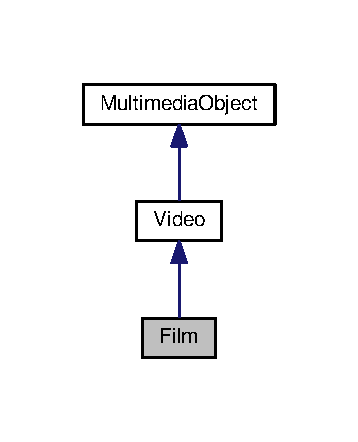
\includegraphics[width=172pt]{classFilm__inherit__graph}
\end{center}
\end{figure}


Collaboration diagram for Film\+:
\nopagebreak
\begin{figure}[H]
\begin{center}
\leavevmode
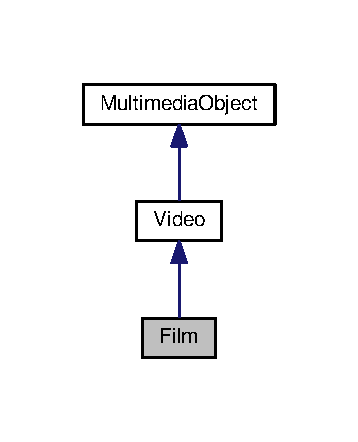
\includegraphics[width=172pt]{classFilm__coll__graph}
\end{center}
\end{figure}
\subsection*{Public Member Functions}
\begin{DoxyCompactItemize}
\item 
virtual \hyperlink{classFilm_a8dab653f8a6c0635ca5ddbe0bbdd9a25}{$\sim$\+Film} ()
\begin{DoxyCompactList}\small\item\em Destroys the film. \end{DoxyCompactList}\item 
\hypertarget{classFilm_af2835db2b0ef3a87aaa3222f4d9d1ae3}{}\hyperlink{classFilm_af2835db2b0ef3a87aaa3222f4d9d1ae3}{Film} ()\label{classFilm_af2835db2b0ef3a87aaa3222f4d9d1ae3}

\begin{DoxyCompactList}\small\item\em Constructs the film. \end{DoxyCompactList}\item 
\hyperlink{classFilm_a49b995034abaf3bea5637def0e4fa506}{Film} (string name, string pathname, int \+\_\+length, int $\ast$\+\_\+chapters, int \+\_\+number\+Of\+Chapters)
\begin{DoxyCompactList}\small\item\em Constructs the film. \end{DoxyCompactList}\item 
int \hyperlink{classFilm_ac089b88c348722506ebbe11f52457e5a}{get\+Number\+Of\+Chapters} () const 
\begin{DoxyCompactList}\small\item\em Gets the number of chapters. \end{DoxyCompactList}\item 
const int $\ast$ \hyperlink{classFilm_a6d5822c887a754ed6c450e8e2805c980}{get\+Chapters} () const 
\begin{DoxyCompactList}\small\item\em Gets the chapters. \end{DoxyCompactList}\item 
string \hyperlink{classFilm_a6e2b00b6a47bd58b925cca372167697c}{get\+Class\+Name} () const override
\begin{DoxyCompactList}\small\item\em Gets the class name. \end{DoxyCompactList}\item 
void \hyperlink{classFilm_ad8f7bea4b733b53a7f0b34b15c68ec95}{set\+Chapters} (const int $\ast$new\+Chapters, int new\+Chapters\+Number)
\begin{DoxyCompactList}\small\item\em Sets the chapters. \end{DoxyCompactList}\item 
void \hyperlink{classFilm_aa0693c2cdbd90495455501f28c85902e}{display\+Chapters} (ostream \&os) const 
\begin{DoxyCompactList}\small\item\em Displays the chapter\textquotesingle{}s length. \end{DoxyCompactList}\item 
void \hyperlink{classFilm_ae18fda84b1c5894c277efb8fe3f8de11}{write} (ostream \&os) const 
\begin{DoxyCompactList}\small\item\em Used to write the film\textquotesingle{}s content, in a file for instance. \end{DoxyCompactList}\item 
void \hyperlink{classFilm_a97a0c42300b580e677eedbdfdf973947}{read} (istream \&is) override
\begin{DoxyCompactList}\small\item\em Used to read the film\textquotesingle{}s content, from a file for instance. \end{DoxyCompactList}\end{DoxyCompactItemize}


\subsection{Detailed Description}
\hyperlink{classFilm}{Film} class, extends the video class. Using pointers for learning purpose. 

\subsection{Constructor \& Destructor Documentation}
\hypertarget{classFilm_a8dab653f8a6c0635ca5ddbe0bbdd9a25}{}\index{Film@{Film}!````~Film@{$\sim$\+Film}}
\index{````~Film@{$\sim$\+Film}!Film@{Film}}
\subsubsection[{$\sim$\+Film}]{\setlength{\rightskip}{0pt plus 5cm}Film\+::$\sim$\+Film (
\begin{DoxyParamCaption}
{}
\end{DoxyParamCaption}
)\hspace{0.3cm}{\ttfamily [virtual]}}\label{classFilm_a8dab653f8a6c0635ca5ddbe0bbdd9a25}


Destroys the film. 

Desctructor useful here \+: we need to delete allocated memory. \hypertarget{classFilm_a49b995034abaf3bea5637def0e4fa506}{}\index{Film@{Film}!Film@{Film}}
\index{Film@{Film}!Film@{Film}}
\subsubsection[{Film}]{\setlength{\rightskip}{0pt plus 5cm}Film\+::\+Film (
\begin{DoxyParamCaption}
\item[{string}]{name, }
\item[{string}]{pathname, }
\item[{int}]{\+\_\+length, }
\item[{int $\ast$}]{\+\_\+chapters, }
\item[{int}]{\+\_\+number\+Of\+Chapters}
\end{DoxyParamCaption}
)}\label{classFilm_a49b995034abaf3bea5637def0e4fa506}


Constructs the film. 


\begin{DoxyParams}[1]{Parameters}
\mbox{\tt in}  & {\em name} & The name \\
\hline
\mbox{\tt in}  & {\em pathname} & The pathname \\
\hline
\mbox{\tt in}  & {\em \+\_\+length} & The length \\
\hline
 & {\em \+\_\+chapters} & The chapters \\
\hline
\mbox{\tt in}  & {\em \+\_\+number\+Of\+Chapters} & The number of chapters \\
\hline
\end{DoxyParams}
std\+::copy\+\_\+n used to make a deep copy. 

\subsection{Member Function Documentation}
\hypertarget{classFilm_aa0693c2cdbd90495455501f28c85902e}{}\index{Film@{Film}!display\+Chapters@{display\+Chapters}}
\index{display\+Chapters@{display\+Chapters}!Film@{Film}}
\subsubsection[{display\+Chapters}]{\setlength{\rightskip}{0pt plus 5cm}void Film\+::display\+Chapters (
\begin{DoxyParamCaption}
\item[{ostream \&}]{os}
\end{DoxyParamCaption}
) const}\label{classFilm_aa0693c2cdbd90495455501f28c85902e}


Displays the chapter\textquotesingle{}s length. 


\begin{DoxyParams}{Parameters}
{\em os} & The ooutput stream. \\
\hline
\end{DoxyParams}
\hypertarget{classFilm_a6d5822c887a754ed6c450e8e2805c980}{}\index{Film@{Film}!get\+Chapters@{get\+Chapters}}
\index{get\+Chapters@{get\+Chapters}!Film@{Film}}
\subsubsection[{get\+Chapters}]{\setlength{\rightskip}{0pt plus 5cm}const int $\ast$ Film\+::get\+Chapters (
\begin{DoxyParamCaption}
{}
\end{DoxyParamCaption}
) const}\label{classFilm_a6d5822c887a754ed6c450e8e2805c980}


Gets the chapters. 

We return a const int$\ast$ for encapsulation sake \+: we don\textquotesingle{}t want the chapters to be changed outside of the class.

\begin{DoxyReturn}{Returns}
The chapters. 
\end{DoxyReturn}
\hypertarget{classFilm_a6e2b00b6a47bd58b925cca372167697c}{}\index{Film@{Film}!get\+Class\+Name@{get\+Class\+Name}}
\index{get\+Class\+Name@{get\+Class\+Name}!Film@{Film}}
\subsubsection[{get\+Class\+Name}]{\setlength{\rightskip}{0pt plus 5cm}string Film\+::get\+Class\+Name (
\begin{DoxyParamCaption}
{}
\end{DoxyParamCaption}
) const\hspace{0.3cm}{\ttfamily [override]}, {\ttfamily [virtual]}}\label{classFilm_a6e2b00b6a47bd58b925cca372167697c}


Gets the class name. 

\begin{DoxyReturn}{Returns}
The class name. 
\end{DoxyReturn}


Reimplemented from \hyperlink{classMultimediaObject_a9eca3c9328fe9141dbdfd571e348aded}{Multimedia\+Object}.

\hypertarget{classFilm_ac089b88c348722506ebbe11f52457e5a}{}\index{Film@{Film}!get\+Number\+Of\+Chapters@{get\+Number\+Of\+Chapters}}
\index{get\+Number\+Of\+Chapters@{get\+Number\+Of\+Chapters}!Film@{Film}}
\subsubsection[{get\+Number\+Of\+Chapters}]{\setlength{\rightskip}{0pt plus 5cm}int Film\+::get\+Number\+Of\+Chapters (
\begin{DoxyParamCaption}
{}
\end{DoxyParamCaption}
) const}\label{classFilm_ac089b88c348722506ebbe11f52457e5a}


Gets the number of chapters. 

\begin{DoxyReturn}{Returns}
The number of chapters. 
\end{DoxyReturn}
\hypertarget{classFilm_a97a0c42300b580e677eedbdfdf973947}{}\index{Film@{Film}!read@{read}}
\index{read@{read}!Film@{Film}}
\subsubsection[{read}]{\setlength{\rightskip}{0pt plus 5cm}void Film\+::read (
\begin{DoxyParamCaption}
\item[{istream \&}]{is}
\end{DoxyParamCaption}
)\hspace{0.3cm}{\ttfamily [override]}, {\ttfamily [virtual]}}\label{classFilm_a97a0c42300b580e677eedbdfdf973947}


Used to read the film\textquotesingle{}s content, from a file for instance. 


\begin{DoxyParams}{Parameters}
{\em is} & The input stream. \\
\hline
\end{DoxyParams}
If we already allocated some memory we free it. 

Reimplemented from \hyperlink{classMultimediaObject_af8689299cabe973f9828a69b84ebbce7}{Multimedia\+Object}.

\hypertarget{classFilm_ad8f7bea4b733b53a7f0b34b15c68ec95}{}\index{Film@{Film}!set\+Chapters@{set\+Chapters}}
\index{set\+Chapters@{set\+Chapters}!Film@{Film}}
\subsubsection[{set\+Chapters}]{\setlength{\rightskip}{0pt plus 5cm}void Film\+::set\+Chapters (
\begin{DoxyParamCaption}
\item[{const int $\ast$}]{new\+Chapters, }
\item[{int}]{new\+Chapters\+Number}
\end{DoxyParamCaption}
)}\label{classFilm_ad8f7bea4b733b53a7f0b34b15c68ec95}


Sets the chapters. 


\begin{DoxyParams}[1]{Parameters}
\mbox{\tt in}  & {\em new\+Chapters} & The new chapters \\
\hline
\mbox{\tt in}  & {\em new\+Chapters\+Number} & The new chapters number \\
\hline
\end{DoxyParams}
If we already allocated some memory we free it.

std\+::copy\+\_\+n used to make a deep copy. \hypertarget{classFilm_ae18fda84b1c5894c277efb8fe3f8de11}{}\index{Film@{Film}!write@{write}}
\index{write@{write}!Film@{Film}}
\subsubsection[{write}]{\setlength{\rightskip}{0pt plus 5cm}void Film\+::write (
\begin{DoxyParamCaption}
\item[{ostream \&}]{os}
\end{DoxyParamCaption}
) const\hspace{0.3cm}{\ttfamily [virtual]}}\label{classFilm_ae18fda84b1c5894c277efb8fe3f8de11}


Used to write the film\textquotesingle{}s content, in a file for instance. 


\begin{DoxyParams}{Parameters}
{\em os} & The output stream. \\
\hline
\end{DoxyParams}


Reimplemented from \hyperlink{classMultimediaObject_af838c533bbfc85230c8569dd16be457b}{Multimedia\+Object}.



The documentation for this class was generated from the following files\+:\begin{DoxyCompactItemize}
\item 
Film.\+h\item 
Film.\+cpp\end{DoxyCompactItemize}

\hypertarget{classGroup}{}\section{Group Class Reference}
\label{classGroup}\index{Group@{Group}}


\hyperlink{classGroup}{Group} class extends the std\+::list class. We store shared\+\_\+ptr of multimedia objects to prevent any memory leak.  




{\ttfamily \#include $<$Group.\+h$>$}



Inheritance diagram for Group\+:
\nopagebreak
\begin{figure}[H]
\begin{center}
\leavevmode
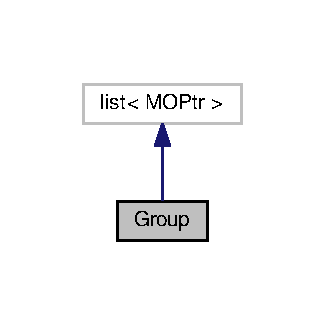
\includegraphics[width=156pt]{classGroup__inherit__graph}
\end{center}
\end{figure}


Collaboration diagram for Group\+:
\nopagebreak
\begin{figure}[H]
\begin{center}
\leavevmode
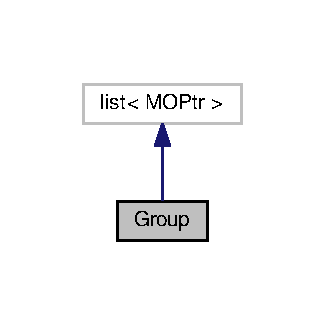
\includegraphics[width=156pt]{classGroup__coll__graph}
\end{center}
\end{figure}
\subsection*{Public Member Functions}
\begin{DoxyCompactItemize}
\item 
\hyperlink{classGroup_aed00a22ff227ee2657ae44a5cbcedf7c}{$\sim$\+Group} ()
\begin{DoxyCompactList}\small\item\em Destroys the group. \end{DoxyCompactList}\item 
\hyperlink{classGroup_a052bee4f590fdd9ed4e6c54cd2575b48}{Group} (string \+\_\+group\+Name)
\begin{DoxyCompactList}\small\item\em Creates the group. \end{DoxyCompactList}\item 
string \hyperlink{classGroup_a59198cfb648e529f61194f14a847e730}{get\+Name} () const 
\begin{DoxyCompactList}\small\item\em Gets the name. \end{DoxyCompactList}\item 
void \hyperlink{classGroup_a9ac8f96722f6e2ea5f666c98306a9579}{display\+Elements} (ostream \&os) const 
\begin{DoxyCompactList}\small\item\em Displays info on all elements of the group. \end{DoxyCompactList}\end{DoxyCompactItemize}


\subsection{Detailed Description}
\hyperlink{classGroup}{Group} class extends the std\+::list class. We store shared\+\_\+ptr of multimedia objects to prevent any memory leak. 

\subsection{Constructor \& Destructor Documentation}
\hypertarget{classGroup_aed00a22ff227ee2657ae44a5cbcedf7c}{}\index{Group@{Group}!````~Group@{$\sim$\+Group}}
\index{````~Group@{$\sim$\+Group}!Group@{Group}}
\subsubsection[{$\sim$\+Group}]{\setlength{\rightskip}{0pt plus 5cm}Group\+::$\sim$\+Group (
\begin{DoxyParamCaption}
{}
\end{DoxyParamCaption}
)}\label{classGroup_aed00a22ff227ee2657ae44a5cbcedf7c}


Destroys the group. 

Destructor used just to keep track of the objects. \hypertarget{classGroup_a052bee4f590fdd9ed4e6c54cd2575b48}{}\index{Group@{Group}!Group@{Group}}
\index{Group@{Group}!Group@{Group}}
\subsubsection[{Group}]{\setlength{\rightskip}{0pt plus 5cm}Group\+::\+Group (
\begin{DoxyParamCaption}
\item[{string}]{\+\_\+group\+Name}
\end{DoxyParamCaption}
)}\label{classGroup_a052bee4f590fdd9ed4e6c54cd2575b48}


Creates the group. 


\begin{DoxyParams}[1]{Parameters}
\mbox{\tt in}  & {\em \+\_\+group\+Name} & The group name \\
\hline
\end{DoxyParams}


\subsection{Member Function Documentation}
\hypertarget{classGroup_a9ac8f96722f6e2ea5f666c98306a9579}{}\index{Group@{Group}!display\+Elements@{display\+Elements}}
\index{display\+Elements@{display\+Elements}!Group@{Group}}
\subsubsection[{display\+Elements}]{\setlength{\rightskip}{0pt plus 5cm}void Group\+::display\+Elements (
\begin{DoxyParamCaption}
\item[{ostream \&}]{os}
\end{DoxyParamCaption}
) const}\label{classGroup_a9ac8f96722f6e2ea5f666c98306a9579}


Displays info on all elements of the group. 


\begin{DoxyParams}{Parameters}
{\em os} & The ouput stream. \\
\hline
\end{DoxyParams}
C++11 like loop \hypertarget{classGroup_a59198cfb648e529f61194f14a847e730}{}\index{Group@{Group}!get\+Name@{get\+Name}}
\index{get\+Name@{get\+Name}!Group@{Group}}
\subsubsection[{get\+Name}]{\setlength{\rightskip}{0pt plus 5cm}string Group\+::get\+Name (
\begin{DoxyParamCaption}
{}
\end{DoxyParamCaption}
) const}\label{classGroup_a59198cfb648e529f61194f14a847e730}


Gets the name. 

\begin{DoxyReturn}{Returns}
The name. 
\end{DoxyReturn}


The documentation for this class was generated from the following files\+:\begin{DoxyCompactItemize}
\item 
Group.\+h\item 
Group.\+cpp\end{DoxyCompactItemize}

\hypertarget{structcppu_1_1InputBuffer}{}\section{cppu\+:\+:Input\+Buffer Struct Reference}
\label{structcppu_1_1InputBuffer}\index{cppu\+::\+Input\+Buffer@{cppu\+::\+Input\+Buffer}}
\subsection*{Public Member Functions}
\begin{DoxyCompactItemize}
\item 
\hypertarget{structcppu_1_1InputBuffer_ac50e17e3cfb76a2983e5e3d4558b8144}{}{\bfseries Input\+Buffer} (size\+\_\+t size)\label{structcppu_1_1InputBuffer_ac50e17e3cfb76a2983e5e3d4558b8144}

\end{DoxyCompactItemize}
\subsection*{Public Attributes}
\begin{DoxyCompactItemize}
\item 
\hypertarget{structcppu_1_1InputBuffer_a85138068e2e10731e46784b1552bc354}{}char $\ast$ {\bfseries buffer}\label{structcppu_1_1InputBuffer_a85138068e2e10731e46784b1552bc354}

\item 
\hypertarget{structcppu_1_1InputBuffer_adbd6fb30fe51a192c9bbba6333016f31}{}char $\ast$ {\bfseries begin}\label{structcppu_1_1InputBuffer_adbd6fb30fe51a192c9bbba6333016f31}

\item 
\hypertarget{structcppu_1_1InputBuffer_ac9fb4f51a6db191e71976fcda20237c0}{}char $\ast$ {\bfseries end}\label{structcppu_1_1InputBuffer_ac9fb4f51a6db191e71976fcda20237c0}

\item 
\hypertarget{structcppu_1_1InputBuffer_a646b547733665524fa8b5de6b093ab11}{}ssize\+\_\+t {\bfseries remaining}\label{structcppu_1_1InputBuffer_a646b547733665524fa8b5de6b093ab11}

\end{DoxyCompactItemize}


The documentation for this struct was generated from the following file\+:\begin{DoxyCompactItemize}
\item 
cpp\+Socket.\+cpp\end{DoxyCompactItemize}

\hypertarget{classMultimediaObject}{}\section{Multimedia\+Object Class Reference}
\label{classMultimediaObject}\index{Multimedia\+Object@{Multimedia\+Object}}


Abstract class for a multimedia object.  




{\ttfamily \#include $<$Multimedia\+Object.\+h$>$}



Inheritance diagram for Multimedia\+Object\+:
\nopagebreak
\begin{figure}[H]
\begin{center}
\leavevmode
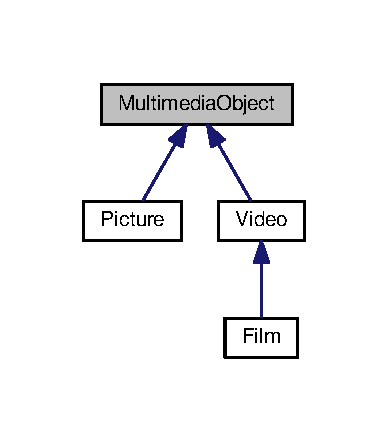
\includegraphics[width=186pt]{classMultimediaObject__inherit__graph}
\end{center}
\end{figure}
\subsection*{Public Member Functions}
\begin{DoxyCompactItemize}
\item 
\hypertarget{classMultimediaObject_a9f24b38d405a785a73660885ede3b9c5}{}virtual \hyperlink{classMultimediaObject_a9f24b38d405a785a73660885ede3b9c5}{$\sim$\+Multimedia\+Object} ()\label{classMultimediaObject_a9f24b38d405a785a73660885ede3b9c5}

\begin{DoxyCompactList}\small\item\em Destroys the object. \end{DoxyCompactList}\item 
\hypertarget{classMultimediaObject_abba8b5f14970dcd1f035c25dd6cdc0bc}{}\hyperlink{classMultimediaObject_abba8b5f14970dcd1f035c25dd6cdc0bc}{Multimedia\+Object} ()\label{classMultimediaObject_abba8b5f14970dcd1f035c25dd6cdc0bc}

\begin{DoxyCompactList}\small\item\em Creates the object. \end{DoxyCompactList}\item 
\hyperlink{classMultimediaObject_ac08b63898b63faedcab9f03fa4d44506}{Multimedia\+Object} (const string \&name, const string \&pathname)
\begin{DoxyCompactList}\small\item\em Creates the object. \end{DoxyCompactList}\item 
string \hyperlink{classMultimediaObject_aef20e4a114ff0013ca01b6477bc0282e}{get\+Name} () const 
\begin{DoxyCompactList}\small\item\em Gets the name. \end{DoxyCompactList}\item 
string \hyperlink{classMultimediaObject_a493f2d99c38a0c835a689cf8a0aca0c3}{get\+Path} () const 
\begin{DoxyCompactList}\small\item\em Gets the path. \end{DoxyCompactList}\item 
virtual string \hyperlink{classMultimediaObject_a9eca3c9328fe9141dbdfd571e348aded}{get\+Class\+Name} () const 
\begin{DoxyCompactList}\small\item\em Gets the class name. \end{DoxyCompactList}\item 
void \hyperlink{classMultimediaObject_ad8b8d859412978bd6bbcacedf8f5a2fa}{set\+Name} (const string \&\+\_\+name)
\begin{DoxyCompactList}\small\item\em Sets the name. \end{DoxyCompactList}\item 
void \hyperlink{classMultimediaObject_abf9ff0aa53c66fd18e87bd5d5739e70e}{set\+Path} (const string \&\+\_\+pathname)
\begin{DoxyCompactList}\small\item\em Sets the path. \end{DoxyCompactList}\item 
virtual void \hyperlink{classMultimediaObject_a9249406bc68f3aea92c87744c3f657da}{display} (ostream \&os) const 
\begin{DoxyCompactList}\small\item\em Displays info on the object. \end{DoxyCompactList}\item 
\hypertarget{classMultimediaObject_a4fc54cf0e9fe39e1b885f995f49f9194}{}virtual void \hyperlink{classMultimediaObject_a4fc54cf0e9fe39e1b885f995f49f9194}{play} () const =0\label{classMultimediaObject_a4fc54cf0e9fe39e1b885f995f49f9194}

\begin{DoxyCompactList}\small\item\em Plays the object. This method is abstract. \end{DoxyCompactList}\item 
virtual void \hyperlink{classMultimediaObject_af838c533bbfc85230c8569dd16be457b}{write} (ostream \&os) const 
\begin{DoxyCompactList}\small\item\em Used to write the object\textquotesingle{}s content, in a file for instance. \end{DoxyCompactList}\item 
virtual void \hyperlink{classMultimediaObject_af8689299cabe973f9828a69b84ebbce7}{read} (istream \&is)
\begin{DoxyCompactList}\small\item\em Used to read the object\textquotesingle{}s content, from a file for instance. \end{DoxyCompactList}\end{DoxyCompactItemize}


\subsection{Detailed Description}
Abstract class for a multimedia object. 

\subsection{Constructor \& Destructor Documentation}
\hypertarget{classMultimediaObject_ac08b63898b63faedcab9f03fa4d44506}{}\index{Multimedia\+Object@{Multimedia\+Object}!Multimedia\+Object@{Multimedia\+Object}}
\index{Multimedia\+Object@{Multimedia\+Object}!Multimedia\+Object@{Multimedia\+Object}}
\subsubsection[{Multimedia\+Object}]{\setlength{\rightskip}{0pt plus 5cm}mo\+::\+Multimedia\+Object (
\begin{DoxyParamCaption}
\item[{const string \&}]{name, }
\item[{const string \&}]{pathname}
\end{DoxyParamCaption}
)}\label{classMultimediaObject_ac08b63898b63faedcab9f03fa4d44506}


Creates the object. 


\begin{DoxyParams}[1]{Parameters}
\mbox{\tt in}  & {\em name} & The name \\
\hline
\mbox{\tt in}  & {\em pathname} & The pathname \\
\hline
\end{DoxyParams}


\subsection{Member Function Documentation}
\hypertarget{classMultimediaObject_a9249406bc68f3aea92c87744c3f657da}{}\index{Multimedia\+Object@{Multimedia\+Object}!display@{display}}
\index{display@{display}!Multimedia\+Object@{Multimedia\+Object}}
\subsubsection[{display}]{\setlength{\rightskip}{0pt plus 5cm}void mo\+::display (
\begin{DoxyParamCaption}
\item[{ostream \&}]{os}
\end{DoxyParamCaption}
) const\hspace{0.3cm}{\ttfamily [virtual]}}\label{classMultimediaObject_a9249406bc68f3aea92c87744c3f657da}


Displays info on the object. 


\begin{DoxyParams}{Parameters}
{\em os} & The output stream. \\
\hline
\end{DoxyParams}


Reimplemented in \hyperlink{classPicture_ac9ec4fc3fe578eeb6f22ce82ab32bc6a}{Picture}, and \hyperlink{classVideo_a8acaac2f61e1989cf3a7dcafd14d8daf}{Video}.

\hypertarget{classMultimediaObject_a9eca3c9328fe9141dbdfd571e348aded}{}\index{Multimedia\+Object@{Multimedia\+Object}!get\+Class\+Name@{get\+Class\+Name}}
\index{get\+Class\+Name@{get\+Class\+Name}!Multimedia\+Object@{Multimedia\+Object}}
\subsubsection[{get\+Class\+Name}]{\setlength{\rightskip}{0pt plus 5cm}string mo\+::get\+Class\+Name (
\begin{DoxyParamCaption}
{}
\end{DoxyParamCaption}
) const\hspace{0.3cm}{\ttfamily [virtual]}}\label{classMultimediaObject_a9eca3c9328fe9141dbdfd571e348aded}


Gets the class name. 

\begin{DoxyReturn}{Returns}
The class name. 
\end{DoxyReturn}


Reimplemented in \hyperlink{classFilm_a6e2b00b6a47bd58b925cca372167697c}{Film}, \hyperlink{classPicture_a91c2c1237c8bef245be245ea8aa6ef82}{Picture}, and \hyperlink{classVideo_a675d26365c71c29bc4b4b50ec2b36bc6}{Video}.

\hypertarget{classMultimediaObject_aef20e4a114ff0013ca01b6477bc0282e}{}\index{Multimedia\+Object@{Multimedia\+Object}!get\+Name@{get\+Name}}
\index{get\+Name@{get\+Name}!Multimedia\+Object@{Multimedia\+Object}}
\subsubsection[{get\+Name}]{\setlength{\rightskip}{0pt plus 5cm}string mo\+::get\+Name (
\begin{DoxyParamCaption}
{}
\end{DoxyParamCaption}
) const}\label{classMultimediaObject_aef20e4a114ff0013ca01b6477bc0282e}


Gets the name. 

\begin{DoxyReturn}{Returns}
The name. 
\end{DoxyReturn}
\hypertarget{classMultimediaObject_a493f2d99c38a0c835a689cf8a0aca0c3}{}\index{Multimedia\+Object@{Multimedia\+Object}!get\+Path@{get\+Path}}
\index{get\+Path@{get\+Path}!Multimedia\+Object@{Multimedia\+Object}}
\subsubsection[{get\+Path}]{\setlength{\rightskip}{0pt plus 5cm}string mo\+::get\+Path (
\begin{DoxyParamCaption}
{}
\end{DoxyParamCaption}
) const}\label{classMultimediaObject_a493f2d99c38a0c835a689cf8a0aca0c3}


Gets the path. 

\begin{DoxyReturn}{Returns}
The path. 
\end{DoxyReturn}
\hypertarget{classMultimediaObject_af8689299cabe973f9828a69b84ebbce7}{}\index{Multimedia\+Object@{Multimedia\+Object}!read@{read}}
\index{read@{read}!Multimedia\+Object@{Multimedia\+Object}}
\subsubsection[{read}]{\setlength{\rightskip}{0pt plus 5cm}void mo\+::read (
\begin{DoxyParamCaption}
\item[{istream \&}]{is}
\end{DoxyParamCaption}
)\hspace{0.3cm}{\ttfamily [virtual]}}\label{classMultimediaObject_af8689299cabe973f9828a69b84ebbce7}


Used to read the object\textquotesingle{}s content, from a file for instance. 


\begin{DoxyParams}{Parameters}
{\em is} & The input stream. \\
\hline
\end{DoxyParams}
We use getline so that we don\textquotesingle{}t stop at the first space encountered. 

Reimplemented in \hyperlink{classPicture_a5d47e31992676d32a7fda30fbb3d3643}{Picture}, \hyperlink{classFilm_a97a0c42300b580e677eedbdfdf973947}{Film}, and \hyperlink{classVideo_a82ebc9192a50d9235f733a50f6710951}{Video}.

\hypertarget{classMultimediaObject_ad8b8d859412978bd6bbcacedf8f5a2fa}{}\index{Multimedia\+Object@{Multimedia\+Object}!set\+Name@{set\+Name}}
\index{set\+Name@{set\+Name}!Multimedia\+Object@{Multimedia\+Object}}
\subsubsection[{set\+Name}]{\setlength{\rightskip}{0pt plus 5cm}void mo\+::set\+Name (
\begin{DoxyParamCaption}
\item[{const string \&}]{\+\_\+name}
\end{DoxyParamCaption}
)}\label{classMultimediaObject_ad8b8d859412978bd6bbcacedf8f5a2fa}


Sets the name. 


\begin{DoxyParams}[1]{Parameters}
\mbox{\tt in}  & {\em \+\_\+name} & The name \\
\hline
\end{DoxyParams}
\hypertarget{classMultimediaObject_abf9ff0aa53c66fd18e87bd5d5739e70e}{}\index{Multimedia\+Object@{Multimedia\+Object}!set\+Path@{set\+Path}}
\index{set\+Path@{set\+Path}!Multimedia\+Object@{Multimedia\+Object}}
\subsubsection[{set\+Path}]{\setlength{\rightskip}{0pt plus 5cm}void mo\+::set\+Path (
\begin{DoxyParamCaption}
\item[{const string \&}]{\+\_\+pathname}
\end{DoxyParamCaption}
)}\label{classMultimediaObject_abf9ff0aa53c66fd18e87bd5d5739e70e}


Sets the path. 


\begin{DoxyParams}[1]{Parameters}
\mbox{\tt in}  & {\em \+\_\+pathname} & The pathname \\
\hline
\end{DoxyParams}
\hypertarget{classMultimediaObject_af838c533bbfc85230c8569dd16be457b}{}\index{Multimedia\+Object@{Multimedia\+Object}!write@{write}}
\index{write@{write}!Multimedia\+Object@{Multimedia\+Object}}
\subsubsection[{write}]{\setlength{\rightskip}{0pt plus 5cm}void mo\+::write (
\begin{DoxyParamCaption}
\item[{ostream \&}]{os}
\end{DoxyParamCaption}
) const\hspace{0.3cm}{\ttfamily [virtual]}}\label{classMultimediaObject_af838c533bbfc85230c8569dd16be457b}


Used to write the object\textquotesingle{}s content, in a file for instance. 


\begin{DoxyParams}{Parameters}
{\em os} & The output stream. \\
\hline
\end{DoxyParams}


Reimplemented in \hyperlink{classPicture_ac54200304abe61c179262f54747b6691}{Picture}, \hyperlink{classFilm_ae18fda84b1c5894c277efb8fe3f8de11}{Film}, and \hyperlink{classVideo_ae71c8af72630d7d145bd948121aac01b}{Video}.



The documentation for this class was generated from the following files\+:\begin{DoxyCompactItemize}
\item 
Multimedia\+Object.\+h\item 
Multimedia\+Object.\+cpp\end{DoxyCompactItemize}

\hypertarget{classPicture}{}\section{Picture Class Reference}
\label{classPicture}\index{Picture@{Picture}}


\hyperlink{classPicture}{Picture} class, extends the abstract class \hyperlink{classMultimediaObject}{Multimedia\+Object}.  




{\ttfamily \#include $<$Picture.\+h$>$}



Inheritance diagram for Picture\+:
\nopagebreak
\begin{figure}[H]
\begin{center}
\leavevmode
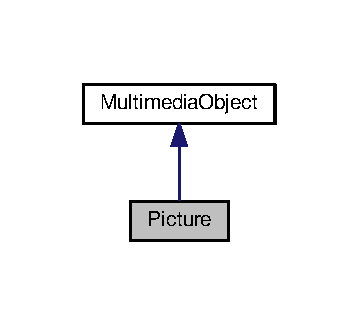
\includegraphics[width=172pt]{classPicture__inherit__graph}
\end{center}
\end{figure}


Collaboration diagram for Picture\+:
\nopagebreak
\begin{figure}[H]
\begin{center}
\leavevmode
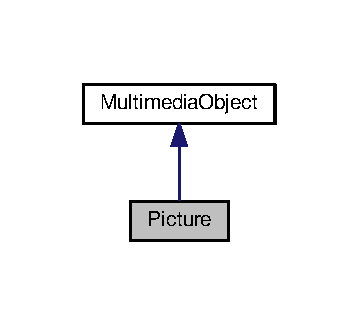
\includegraphics[width=172pt]{classPicture__coll__graph}
\end{center}
\end{figure}
\subsection*{Public Member Functions}
\begin{DoxyCompactItemize}
\item 
virtual \hyperlink{classPicture_af09bc804565eb973016527ff720ee504}{$\sim$\+Picture} ()
\begin{DoxyCompactList}\small\item\em Destroys the picture. \end{DoxyCompactList}\item 
\hypertarget{classPicture_ae71db353784869ca50fd695c6c89c9f3}{}\hyperlink{classPicture_ae71db353784869ca50fd695c6c89c9f3}{Picture} ()\label{classPicture_ae71db353784869ca50fd695c6c89c9f3}

\begin{DoxyCompactList}\small\item\em Constructs the picture. \end{DoxyCompactList}\item 
\hyperlink{classPicture_a5a385595e86d57a60fc3ee0deac7a434}{Picture} (const string \&name, const string \&pathname, const double \&\+\_\+latitude, const double \&\+\_\+longitude)
\begin{DoxyCompactList}\small\item\em Constructs the picture. \end{DoxyCompactList}\item 
double \hyperlink{classPicture_aa1ee860b82a140bfb1c83217d06f2cd7}{get\+Latitude} () const 
\begin{DoxyCompactList}\small\item\em Gets the latitude. \end{DoxyCompactList}\item 
double \hyperlink{classPicture_a5c26ca5c555d29735c7dfa5cdfa83286}{get\+Longitude} () const 
\begin{DoxyCompactList}\small\item\em Gets the longitude. \end{DoxyCompactList}\item 
string \hyperlink{classPicture_a91c2c1237c8bef245be245ea8aa6ef82}{get\+Class\+Name} () const override
\begin{DoxyCompactList}\small\item\em Gets the class name. \end{DoxyCompactList}\item 
void \hyperlink{classPicture_af4d86c3c40c1b6a6450a14f3f13da1a4}{set\+Latitude} (const double \&\+\_\+latitude)
\begin{DoxyCompactList}\small\item\em Sets the latitude. \end{DoxyCompactList}\item 
void \hyperlink{classPicture_a3f0d272d5df7dfcbb1cfa9a216a05134}{set\+Longitude} (const double \&\+\_\+longitude)
\begin{DoxyCompactList}\small\item\em Sets the longitude. \end{DoxyCompactList}\item 
void \hyperlink{classPicture_ac9ec4fc3fe578eeb6f22ce82ab32bc6a}{display} (ostream \&os) const override
\begin{DoxyCompactList}\small\item\em Displays info on the picture. \end{DoxyCompactList}\item 
\hypertarget{classPicture_a9c3aab87ad22bf2020c50fa3e1845e40}{}void \hyperlink{classPicture_a9c3aab87ad22bf2020c50fa3e1845e40}{play} () const override\label{classPicture_a9c3aab87ad22bf2020c50fa3e1845e40}

\begin{DoxyCompactList}\small\item\em Shows the picture using imagej.\+S. \end{DoxyCompactList}\item 
void \hyperlink{classPicture_ac54200304abe61c179262f54747b6691}{write} (ostream \&os) const override
\begin{DoxyCompactList}\small\item\em Used to write the picture\textquotesingle{}s content, in a file for instance. \end{DoxyCompactList}\item 
void \hyperlink{classPicture_a5d47e31992676d32a7fda30fbb3d3643}{read} (istream \&is) override
\begin{DoxyCompactList}\small\item\em Used to read the video\textquotesingle{}s content, from a file for instance. \end{DoxyCompactList}\end{DoxyCompactItemize}


\subsection{Detailed Description}
\hyperlink{classPicture}{Picture} class, extends the abstract class \hyperlink{classMultimediaObject}{Multimedia\+Object}. 

\subsection{Constructor \& Destructor Documentation}
\hypertarget{classPicture_af09bc804565eb973016527ff720ee504}{}\index{Picture@{Picture}!````~Picture@{$\sim$\+Picture}}
\index{````~Picture@{$\sim$\+Picture}!Picture@{Picture}}
\subsubsection[{$\sim$\+Picture}]{\setlength{\rightskip}{0pt plus 5cm}pic\+::$\sim$\+Picture (
\begin{DoxyParamCaption}
{}
\end{DoxyParamCaption}
)\hspace{0.3cm}{\ttfamily [virtual]}}\label{classPicture_af09bc804565eb973016527ff720ee504}


Destroys the picture. 

Destructor used just to keep track of the objects. \hypertarget{classPicture_a5a385595e86d57a60fc3ee0deac7a434}{}\index{Picture@{Picture}!Picture@{Picture}}
\index{Picture@{Picture}!Picture@{Picture}}
\subsubsection[{Picture}]{\setlength{\rightskip}{0pt plus 5cm}pic\+::\+Picture (
\begin{DoxyParamCaption}
\item[{const string \&}]{name, }
\item[{const string \&}]{pathname, }
\item[{const double \&}]{\+\_\+latitude, }
\item[{const double \&}]{\+\_\+longitude}
\end{DoxyParamCaption}
)}\label{classPicture_a5a385595e86d57a60fc3ee0deac7a434}


Constructs the picture. 


\begin{DoxyParams}[1]{Parameters}
\mbox{\tt in}  & {\em name} & The name \\
\hline
\mbox{\tt in}  & {\em pathname} & The pathname \\
\hline
\mbox{\tt in}  & {\em \+\_\+latitude} & The latitude \\
\hline
\mbox{\tt in}  & {\em \+\_\+longitude} & The longitude \\
\hline
\end{DoxyParams}


\subsection{Member Function Documentation}
\hypertarget{classPicture_ac9ec4fc3fe578eeb6f22ce82ab32bc6a}{}\index{Picture@{Picture}!display@{display}}
\index{display@{display}!Picture@{Picture}}
\subsubsection[{display}]{\setlength{\rightskip}{0pt plus 5cm}void pic\+::display (
\begin{DoxyParamCaption}
\item[{ostream \&}]{os}
\end{DoxyParamCaption}
) const\hspace{0.3cm}{\ttfamily [override]}, {\ttfamily [virtual]}}\label{classPicture_ac9ec4fc3fe578eeb6f22ce82ab32bc6a}


Displays info on the picture. 


\begin{DoxyParams}{Parameters}
{\em os} & The output stream \\
\hline
\end{DoxyParams}


Reimplemented from \hyperlink{classMultimediaObject_a9249406bc68f3aea92c87744c3f657da}{Multimedia\+Object}.

\hypertarget{classPicture_a91c2c1237c8bef245be245ea8aa6ef82}{}\index{Picture@{Picture}!get\+Class\+Name@{get\+Class\+Name}}
\index{get\+Class\+Name@{get\+Class\+Name}!Picture@{Picture}}
\subsubsection[{get\+Class\+Name}]{\setlength{\rightskip}{0pt plus 5cm}string pic\+::get\+Class\+Name (
\begin{DoxyParamCaption}
{}
\end{DoxyParamCaption}
) const\hspace{0.3cm}{\ttfamily [override]}, {\ttfamily [virtual]}}\label{classPicture_a91c2c1237c8bef245be245ea8aa6ef82}


Gets the class name. 

\begin{DoxyReturn}{Returns}
The class name. 
\end{DoxyReturn}


Reimplemented from \hyperlink{classMultimediaObject_a9eca3c9328fe9141dbdfd571e348aded}{Multimedia\+Object}.

\hypertarget{classPicture_aa1ee860b82a140bfb1c83217d06f2cd7}{}\index{Picture@{Picture}!get\+Latitude@{get\+Latitude}}
\index{get\+Latitude@{get\+Latitude}!Picture@{Picture}}
\subsubsection[{get\+Latitude}]{\setlength{\rightskip}{0pt plus 5cm}double pic\+::get\+Latitude (
\begin{DoxyParamCaption}
{}
\end{DoxyParamCaption}
) const}\label{classPicture_aa1ee860b82a140bfb1c83217d06f2cd7}


Gets the latitude. 

\begin{DoxyReturn}{Returns}
The latitude. 
\end{DoxyReturn}
\hypertarget{classPicture_a5c26ca5c555d29735c7dfa5cdfa83286}{}\index{Picture@{Picture}!get\+Longitude@{get\+Longitude}}
\index{get\+Longitude@{get\+Longitude}!Picture@{Picture}}
\subsubsection[{get\+Longitude}]{\setlength{\rightskip}{0pt plus 5cm}double pic\+::get\+Longitude (
\begin{DoxyParamCaption}
{}
\end{DoxyParamCaption}
) const}\label{classPicture_a5c26ca5c555d29735c7dfa5cdfa83286}


Gets the longitude. 

\begin{DoxyReturn}{Returns}
The longitude. 
\end{DoxyReturn}
\hypertarget{classPicture_a5d47e31992676d32a7fda30fbb3d3643}{}\index{Picture@{Picture}!read@{read}}
\index{read@{read}!Picture@{Picture}}
\subsubsection[{read}]{\setlength{\rightskip}{0pt plus 5cm}void pic\+::read (
\begin{DoxyParamCaption}
\item[{istream \&}]{is}
\end{DoxyParamCaption}
)\hspace{0.3cm}{\ttfamily [override]}, {\ttfamily [virtual]}}\label{classPicture_a5d47e31992676d32a7fda30fbb3d3643}


Used to read the video\textquotesingle{}s content, from a file for instance. 


\begin{DoxyParams}{Parameters}
{\em is} & The input stream. \\
\hline
\end{DoxyParams}


Reimplemented from \hyperlink{classMultimediaObject_af8689299cabe973f9828a69b84ebbce7}{Multimedia\+Object}.

\hypertarget{classPicture_af4d86c3c40c1b6a6450a14f3f13da1a4}{}\index{Picture@{Picture}!set\+Latitude@{set\+Latitude}}
\index{set\+Latitude@{set\+Latitude}!Picture@{Picture}}
\subsubsection[{set\+Latitude}]{\setlength{\rightskip}{0pt plus 5cm}void pic\+::set\+Latitude (
\begin{DoxyParamCaption}
\item[{const double \&}]{\+\_\+latitude}
\end{DoxyParamCaption}
)}\label{classPicture_af4d86c3c40c1b6a6450a14f3f13da1a4}


Sets the latitude. 


\begin{DoxyParams}[1]{Parameters}
\mbox{\tt in}  & {\em \+\_\+latitude} & The latitude \\
\hline
\end{DoxyParams}
\hypertarget{classPicture_a3f0d272d5df7dfcbb1cfa9a216a05134}{}\index{Picture@{Picture}!set\+Longitude@{set\+Longitude}}
\index{set\+Longitude@{set\+Longitude}!Picture@{Picture}}
\subsubsection[{set\+Longitude}]{\setlength{\rightskip}{0pt plus 5cm}void pic\+::set\+Longitude (
\begin{DoxyParamCaption}
\item[{const double \&}]{\+\_\+longitude}
\end{DoxyParamCaption}
)}\label{classPicture_a3f0d272d5df7dfcbb1cfa9a216a05134}


Sets the longitude. 


\begin{DoxyParams}[1]{Parameters}
\mbox{\tt in}  & {\em \+\_\+longitude} & The longitude \\
\hline
\end{DoxyParams}
\hypertarget{classPicture_ac54200304abe61c179262f54747b6691}{}\index{Picture@{Picture}!write@{write}}
\index{write@{write}!Picture@{Picture}}
\subsubsection[{write}]{\setlength{\rightskip}{0pt plus 5cm}void pic\+::write (
\begin{DoxyParamCaption}
\item[{ostream \&}]{os}
\end{DoxyParamCaption}
) const\hspace{0.3cm}{\ttfamily [override]}, {\ttfamily [virtual]}}\label{classPicture_ac54200304abe61c179262f54747b6691}


Used to write the picture\textquotesingle{}s content, in a file for instance. 


\begin{DoxyParams}{Parameters}
{\em os} & The output stream. \\
\hline
\end{DoxyParams}


Reimplemented from \hyperlink{classMultimediaObject_af838c533bbfc85230c8569dd16be457b}{Multimedia\+Object}.



The documentation for this class was generated from the following files\+:\begin{DoxyCompactItemize}
\item 
Picture.\+h\item 
Picture.\+cpp\end{DoxyCompactItemize}

\hypertarget{classcppu_1_1ServerSocket}{}\section{cppu\+:\+:Server\+Socket Class Reference}
\label{classcppu_1_1ServerSocket}\index{cppu\+::\+Server\+Socket@{cppu\+::\+Server\+Socket}}


T\+C\+P/\+I\+P server socket. This class implements a T\+C\+P/\+I\+P socket that waits for requests to come in over the network. A\+F\+\_\+\+I\+N\+E\+T connections following the I\+Pv4 Internet protocol are supported.  




{\ttfamily \#include $<$cpp\+Socket.\+h$>$}

\subsection*{Public Member Functions}
\begin{DoxyCompactItemize}
\item 
\hypertarget{classcppu_1_1ServerSocket_a57138f5a7d2e8af35228c8985385c494}{}\hyperlink{classcppu_1_1ServerSocket_a57138f5a7d2e8af35228c8985385c494}{Server\+Socket} ()\label{classcppu_1_1ServerSocket_a57138f5a7d2e8af35228c8985385c494}

\begin{DoxyCompactList}\small\item\em Creates a new server socket. Creates a listening socket that waits for connection requests by T\+C\+P/\+I\+P clients. \end{DoxyCompactList}\item 
virtual \hyperlink{classcppu_1_1Socket}{Socket} $\ast$ \hyperlink{classcppu_1_1ServerSocket_af08ebcb886fc778d195fb622f7b96b8b}{accept} ()
\begin{DoxyCompactList}\small\item\em Accepts a new connection request and returns the corresponding socket. By default, this function blocks the caller until a connection is present. \end{DoxyCompactList}\item 
virtual int \hyperlink{classcppu_1_1ServerSocket_a255dfdccba51c7cdbcb6733c6c3f6ffa}{bind} (int port, int backlog=50)
\begin{DoxyCompactList}\small\item\em Assigns the socket to the local address. The socket must be bound before using it. \end{DoxyCompactList}\item 
\hypertarget{classcppu_1_1ServerSocket_ae7647cfb5beaf504a846f6ecfdd197c4}{}virtual int \hyperlink{classcppu_1_1ServerSocket_ae7647cfb5beaf504a846f6ecfdd197c4}{close} ()\label{classcppu_1_1ServerSocket_ae7647cfb5beaf504a846f6ecfdd197c4}

\begin{DoxyCompactList}\small\item\em Closes the socket. \end{DoxyCompactList}\item 
\hypertarget{classcppu_1_1ServerSocket_aa3ca8fed354955eeb45af3a2021c04cb}{}bool \hyperlink{classcppu_1_1ServerSocket_aa3ca8fed354955eeb45af3a2021c04cb}{is\+Closed} () const \label{classcppu_1_1ServerSocket_aa3ca8fed354955eeb45af3a2021c04cb}

\begin{DoxyCompactList}\small\item\em Returns true if the socket has been closed. \end{DoxyCompactList}\item 
\hypertarget{classcppu_1_1ServerSocket_a905d85f63fdca46ed5ee44eb00e211d1}{}int \hyperlink{classcppu_1_1ServerSocket_a905d85f63fdca46ed5ee44eb00e211d1}{descriptor} ()\label{classcppu_1_1ServerSocket_a905d85f63fdca46ed5ee44eb00e211d1}

\begin{DoxyCompactList}\small\item\em Returns the Unix descriptor of the socket. \end{DoxyCompactList}\item 
\hypertarget{classcppu_1_1ServerSocket_a0fbd0ee42bcfecf2e749279c4b94b0b3}{}int \hyperlink{classcppu_1_1ServerSocket_a0fbd0ee42bcfecf2e749279c4b94b0b3}{set\+Receive\+Buffer\+Size} (int size)\label{classcppu_1_1ServerSocket_a0fbd0ee42bcfecf2e749279c4b94b0b3}

\begin{DoxyCompactList}\small\item\em Sets the S\+O\+\_\+\+R\+C\+V\+B\+U\+F option to the specified value. \end{DoxyCompactList}\item 
\hypertarget{classcppu_1_1ServerSocket_a09d0494cc0f65abe496b9c940d2920ed}{}int \hyperlink{classcppu_1_1ServerSocket_a09d0494cc0f65abe496b9c940d2920ed}{set\+Reuse\+Address} (bool)\label{classcppu_1_1ServerSocket_a09d0494cc0f65abe496b9c940d2920ed}

\begin{DoxyCompactList}\small\item\em Enables/disables the S\+O\+\_\+\+R\+E\+U\+S\+E\+A\+D\+D\+R socket option. \end{DoxyCompactList}\item 
\hypertarget{classcppu_1_1ServerSocket_a0ceb984eab0cdd9c7c8e62658a521175}{}int \hyperlink{classcppu_1_1ServerSocket_a0ceb984eab0cdd9c7c8e62658a521175}{set\+So\+Timeout} (int timeout)\label{classcppu_1_1ServerSocket_a0ceb984eab0cdd9c7c8e62658a521175}

\begin{DoxyCompactList}\small\item\em Enables/disables S\+O\+\_\+\+T\+I\+M\+E\+O\+U\+T with the specified timeout (in milliseconds). \end{DoxyCompactList}\item 
\hypertarget{classcppu_1_1ServerSocket_ac5f6da333208cce9ca4d5392259a0a6b}{}int \hyperlink{classcppu_1_1ServerSocket_ac5f6da333208cce9ca4d5392259a0a6b}{set\+Tcp\+No\+Delay} (bool)\label{classcppu_1_1ServerSocket_ac5f6da333208cce9ca4d5392259a0a6b}

\begin{DoxyCompactList}\small\item\em Turns on/off T\+C\+P coalescence (useful in some cases to avoid delays). \end{DoxyCompactList}\end{DoxyCompactItemize}
\subsection*{Protected Member Functions}
\begin{DoxyCompactItemize}
\item 
\hypertarget{classcppu_1_1ServerSocket_a23d038275576d0a969072eb334f7b84f}{}virtual \hyperlink{classcppu_1_1Socket}{Socket} $\ast$ {\bfseries create\+Socket} (int sockfd)\label{classcppu_1_1ServerSocket_a23d038275576d0a969072eb334f7b84f}

\end{DoxyCompactItemize}


\subsection{Detailed Description}
T\+C\+P/\+I\+P server socket. This class implements a T\+C\+P/\+I\+P socket that waits for requests to come in over the network. A\+F\+\_\+\+I\+N\+E\+T connections following the I\+Pv4 Internet protocol are supported. 

\begin{DoxyNote}{Note}
T\+C\+P/\+I\+P sockets do not preserve record boundaries, 
\end{DoxyNote}
\begin{DoxySeeAlso}{See also}
\hyperlink{classcppu_1_1SocketBuffer}{Socket\+Buffer} for a solution. 
\end{DoxySeeAlso}


\subsection{Member Function Documentation}
\hypertarget{classcppu_1_1ServerSocket_af08ebcb886fc778d195fb622f7b96b8b}{}\index{cppu\+::\+Server\+Socket@{cppu\+::\+Server\+Socket}!accept@{accept}}
\index{accept@{accept}!cppu\+::\+Server\+Socket@{cppu\+::\+Server\+Socket}}
\subsubsection[{accept}]{\setlength{\rightskip}{0pt plus 5cm}{\bf Socket} $\ast$ cppu\+::\+Server\+Socket\+::accept (
\begin{DoxyParamCaption}
{}
\end{DoxyParamCaption}
)\hspace{0.3cm}{\ttfamily [virtual]}}\label{classcppu_1_1ServerSocket_af08ebcb886fc778d195fb622f7b96b8b}


Accepts a new connection request and returns the corresponding socket. By default, this function blocks the caller until a connection is present. 

\begin{DoxyReturn}{Returns}
the new \hyperlink{classcppu_1_1Socket}{Socket} or nullptr on error. 
\end{DoxyReturn}
\hypertarget{classcppu_1_1ServerSocket_a255dfdccba51c7cdbcb6733c6c3f6ffa}{}\index{cppu\+::\+Server\+Socket@{cppu\+::\+Server\+Socket}!bind@{bind}}
\index{bind@{bind}!cppu\+::\+Server\+Socket@{cppu\+::\+Server\+Socket}}
\subsubsection[{bind}]{\setlength{\rightskip}{0pt plus 5cm}int cppu\+::\+Server\+Socket\+::bind (
\begin{DoxyParamCaption}
\item[{int}]{port, }
\item[{int}]{backlog = {\ttfamily 50}}
\end{DoxyParamCaption}
)\hspace{0.3cm}{\ttfamily [virtual]}}\label{classcppu_1_1ServerSocket_a255dfdccba51c7cdbcb6733c6c3f6ffa}


Assigns the socket to the local address. The socket must be bound before using it. 

\begin{DoxyReturn}{Returns}
0 on success or a negative value on error which is one of \hyperlink{classcppu_1_1Socket_a49ea5cb079bd7ae97ecf7eb30c9d9e5f}{Socket\+::\+Errors} 
\end{DoxyReturn}


The documentation for this class was generated from the following files\+:\begin{DoxyCompactItemize}
\item 
cpp\+Socket.\+h\item 
cpp\+Socket.\+cpp\end{DoxyCompactItemize}

\hypertarget{classcppu_1_1Socket}{}\section{cppu\+:\+:Socket Class Reference}
\label{classcppu_1_1Socket}\index{cppu\+::\+Socket@{cppu\+::\+Socket}}


T\+C\+P/\+I\+P or U\+D\+P/\+Datagram socket. This class encapsulates a T\+C\+P/\+I\+P or U\+D\+P/\+Datagram socket. A\+F\+\_\+\+I\+N\+E\+T connections following the I\+Pv4 Internet protocol are supported.  




{\ttfamily \#include $<$cpp\+Socket.\+h$>$}

\subsection*{Public Types}
\begin{DoxyCompactItemize}
\item 
enum \hyperlink{classcppu_1_1Socket_a49ea5cb079bd7ae97ecf7eb30c9d9e5f}{Errors} \{ {\bfseries Failed} = -\/1, 
{\bfseries Invalid\+Socket} = -\/2, 
{\bfseries Unknown\+Host} = -\/3
 \}
\begin{DoxyCompactList}\small\item\em \hyperlink{classcppu_1_1Socket}{Socket} errors. \end{DoxyCompactList}\end{DoxyCompactItemize}
\subsection*{Public Member Functions}
\begin{DoxyCompactItemize}
\item 
\hyperlink{classcppu_1_1Socket_ae73b9b629fe443f650203d938f61a279}{Socket} (int type=S\+O\+C\+K\+\_\+\+S\+T\+R\+E\+A\+M)
\begin{DoxyCompactList}\small\item\em Creates a new \hyperlink{classcppu_1_1Socket}{Socket}. Creates a A\+F\+\_\+\+I\+N\+E\+T socket using the I\+Pv4 Internet protocol. Type can be\+: \end{DoxyCompactList}\item 
\hypertarget{classcppu_1_1Socket_a8404e4e80cc625a4be32aacc879bb237}{}\hyperlink{classcppu_1_1Socket_a8404e4e80cc625a4be32aacc879bb237}{Socket} (int type, int sockfd)\label{classcppu_1_1Socket_a8404e4e80cc625a4be32aacc879bb237}

\begin{DoxyCompactList}\small\item\em Creates a \hyperlink{classcppu_1_1Socket}{Socket} object from an existing socket file descriptor. \end{DoxyCompactList}\item 
\hypertarget{classcppu_1_1Socket_ae26733a0b7d8a5fb5544d2d069152de7}{}virtual \hyperlink{classcppu_1_1Socket_ae26733a0b7d8a5fb5544d2d069152de7}{$\sim$\+Socket} ()\label{classcppu_1_1Socket_ae26733a0b7d8a5fb5544d2d069152de7}

\begin{DoxyCompactList}\small\item\em Destructor (closes the socket). \end{DoxyCompactList}\item 
virtual int \hyperlink{classcppu_1_1Socket_a7b876dcaff0babaffde41575f9b19d64}{bind} (int port)
\begin{DoxyCompactList}\small\item\em Assigns the socket to the local address. Typically used for U\+D\+P/\+Datagram sockets,. \end{DoxyCompactList}\item 
virtual int \hyperlink{classcppu_1_1Socket_a5698a3a7c6c203676c6de5e5559a0a7f}{bind} (const std\+::string \&host, int port)
\begin{DoxyCompactList}\small\item\em Assigns the socket to an address. Typically used for U\+D\+P/\+Datagram sockets,. \end{DoxyCompactList}\item 
virtual int \hyperlink{classcppu_1_1Socket_af6db3840caee709738f0e2a9ff814e5d}{connect} (const std\+::string \&host, int port)
\begin{DoxyCompactList}\small\item\em Connects the socket to an address. Typically used for T\+C\+P/\+I\+P sockets on the client side,. \end{DoxyCompactList}\item 
virtual int \hyperlink{classcppu_1_1Socket_ab958ef8a0f0495cf3a1c57a2ad4a34fc}{close} ()
\begin{DoxyCompactList}\small\item\em Closes the socket. \end{DoxyCompactList}\item 
\hypertarget{classcppu_1_1Socket_a726c2e6be413fe4e0584a23a173ae540}{}bool \hyperlink{classcppu_1_1Socket_a726c2e6be413fe4e0584a23a173ae540}{is\+Closed} () const \label{classcppu_1_1Socket_a726c2e6be413fe4e0584a23a173ae540}

\begin{DoxyCompactList}\small\item\em Returns true if the socket has been closed. \end{DoxyCompactList}\item 
\hypertarget{classcppu_1_1Socket_a06a8fcd9518e6a3e8b33bb64f7fb9036}{}int \hyperlink{classcppu_1_1Socket_a06a8fcd9518e6a3e8b33bb64f7fb9036}{descriptor} ()\label{classcppu_1_1Socket_a06a8fcd9518e6a3e8b33bb64f7fb9036}

\begin{DoxyCompactList}\small\item\em Returns the Unix descriptor of the socket. \end{DoxyCompactList}\item 
ssize\+\_\+t \hyperlink{classcppu_1_1Socket_aeac77f859159715e2d63a5a0dc118788}{send} (const void $\ast$buf, size\+\_\+t len, int flags=0)
\begin{DoxyCompactList}\small\item\em Sends data to a connected socket. Sends {\itshape len} bytes to a T\+C\+P/\+I\+P socket using the Unix \hyperlink{classcppu_1_1Socket_aeac77f859159715e2d63a5a0dc118788}{send()} function (. \end{DoxyCompactList}\item 
ssize\+\_\+t \hyperlink{classcppu_1_1Socket_a37c382af52cc02f92c0e19a0c6e0e04f}{receive} (void $\ast$buf, size\+\_\+t len, int flags=0)
\begin{DoxyCompactList}\small\item\em Receives data from a connected socket. Reads at most {\itshape len} bytes from a T\+C\+P/\+I\+P socket using the Unix recv() function. By default, this function blocks the caller until data is present (. \end{DoxyCompactList}\item 
ssize\+\_\+t \hyperlink{classcppu_1_1Socket_a31ff5137959aa4e52d4bcdd53e0b0069}{send\+To} (const void $\ast$buf, size\+\_\+t len, int flags, const struct sockaddr $\ast$dest\+\_\+addr, socklen\+\_\+t addrlen)
\begin{DoxyCompactList}\small\item\em Sends data to a datagram socket. Sends {\itshape len} bytes to a datagram socket using the Unix sendto() function. \end{DoxyCompactList}\item 
ssize\+\_\+t \hyperlink{classcppu_1_1Socket_abd460be82deeb29e730fc83f871e51c4}{receive\+From} (void $\ast$buf, size\+\_\+t len, int flags, struct sockaddr $\ast$src\+\_\+addr, socklen\+\_\+t $\ast$addrlen)
\begin{DoxyCompactList}\small\item\em Receives data from datagram socket. Reads at most {\itshape len} bytes from a datagram socket using the Unix recvfrom() function. By default, this function blocks the caller until data is present (. \end{DoxyCompactList}\item 
\hypertarget{classcppu_1_1Socket_a06c6838f267e5a0ba74558da946efb90}{}virtual void \hyperlink{classcppu_1_1Socket_a06c6838f267e5a0ba74558da946efb90}{shutdown\+Input} ()\label{classcppu_1_1Socket_a06c6838f267e5a0ba74558da946efb90}

\begin{DoxyCompactList}\small\item\em Disables further receive operations. \end{DoxyCompactList}\item 
\hypertarget{classcppu_1_1Socket_a97ee9ef3bf9fdecd6ae6f2b583b34d0e}{}virtual void \hyperlink{classcppu_1_1Socket_a97ee9ef3bf9fdecd6ae6f2b583b34d0e}{shutdown\+Output} ()\label{classcppu_1_1Socket_a97ee9ef3bf9fdecd6ae6f2b583b34d0e}

\begin{DoxyCompactList}\small\item\em Disables further send operations. \end{DoxyCompactList}\item 
\hypertarget{classcppu_1_1Socket_af172d5c78f63713988b0a6bf66851be7}{}int \hyperlink{classcppu_1_1Socket_af172d5c78f63713988b0a6bf66851be7}{set\+Receive\+Buffer\+Size} (int size)\label{classcppu_1_1Socket_af172d5c78f63713988b0a6bf66851be7}

\begin{DoxyCompactList}\small\item\em Sets the size of the T\+C\+P/\+I\+P input buffer. \end{DoxyCompactList}\item 
\hypertarget{classcppu_1_1Socket_a27b7fe34e172ad1f97c304d2786f624a}{}int \hyperlink{classcppu_1_1Socket_a27b7fe34e172ad1f97c304d2786f624a}{set\+Reuse\+Address} (bool)\label{classcppu_1_1Socket_a27b7fe34e172ad1f97c304d2786f624a}

\begin{DoxyCompactList}\small\item\em Enables/disables the S\+O\+\_\+\+R\+E\+U\+S\+E\+A\+D\+D\+R socket option. \end{DoxyCompactList}\item 
\hypertarget{classcppu_1_1Socket_aefda954454d860fa6a6d41b3d5cd26db}{}int \hyperlink{classcppu_1_1Socket_aefda954454d860fa6a6d41b3d5cd26db}{set\+Send\+Buffer\+Size} (int size)\label{classcppu_1_1Socket_aefda954454d860fa6a6d41b3d5cd26db}

\begin{DoxyCompactList}\small\item\em Sets the size of the T\+C\+P/\+I\+P output buffer. \end{DoxyCompactList}\item 
\hypertarget{classcppu_1_1Socket_ae87eb0335c072f765bf2b6a47162e7f5}{}int \hyperlink{classcppu_1_1Socket_ae87eb0335c072f765bf2b6a47162e7f5}{set\+So\+Linger} (bool, int linger)\label{classcppu_1_1Socket_ae87eb0335c072f765bf2b6a47162e7f5}

\begin{DoxyCompactList}\small\item\em Enables/disables S\+O\+\_\+\+L\+I\+N\+G\+E\+R with the specified linger time in seconds. \end{DoxyCompactList}\item 
\hypertarget{classcppu_1_1Socket_ae5dea30a1cae2dbdbdaf11a9f7ffa444}{}int \hyperlink{classcppu_1_1Socket_ae5dea30a1cae2dbdbdaf11a9f7ffa444}{set\+So\+Timeout} (int timeout)\label{classcppu_1_1Socket_ae5dea30a1cae2dbdbdaf11a9f7ffa444}

\begin{DoxyCompactList}\small\item\em Enables/disables S\+O\+\_\+\+T\+I\+M\+E\+O\+U\+T with the specified timeout (in milliseconds). \end{DoxyCompactList}\item 
\hypertarget{classcppu_1_1Socket_a6b29a9e12926b07f65b8dc52176131c5}{}int \hyperlink{classcppu_1_1Socket_a6b29a9e12926b07f65b8dc52176131c5}{set\+Tcp\+No\+Delay} (bool)\label{classcppu_1_1Socket_a6b29a9e12926b07f65b8dc52176131c5}

\begin{DoxyCompactList}\small\item\em Enables/disables T\+C\+P\+\_\+\+N\+O\+D\+E\+L\+A\+Y (turns on/off T\+C\+P coalescence). \end{DoxyCompactList}\item 
\hypertarget{classcppu_1_1Socket_a677726fbe23c7b4117c648d54fd217a4}{}int \hyperlink{classcppu_1_1Socket_a677726fbe23c7b4117c648d54fd217a4}{get\+Receive\+Buffer\+Size} () const \label{classcppu_1_1Socket_a677726fbe23c7b4117c648d54fd217a4}

\begin{DoxyCompactList}\small\item\em Gets the size of the T\+C\+P/\+I\+P input buffer. \end{DoxyCompactList}\item 
\hypertarget{classcppu_1_1Socket_a8b16f99014bf2050394f34b4f0963e8f}{}bool \hyperlink{classcppu_1_1Socket_a8b16f99014bf2050394f34b4f0963e8f}{get\+Reuse\+Address} () const \label{classcppu_1_1Socket_a8b16f99014bf2050394f34b4f0963e8f}

\begin{DoxyCompactList}\small\item\em Gets S\+O\+\_\+\+R\+E\+U\+S\+E\+A\+D\+D\+R state. \end{DoxyCompactList}\item 
\hypertarget{classcppu_1_1Socket_a98fe83074255461c25ac72fcfa974404}{}int \hyperlink{classcppu_1_1Socket_a98fe83074255461c25ac72fcfa974404}{get\+Send\+Buffer\+Size} () const \label{classcppu_1_1Socket_a98fe83074255461c25ac72fcfa974404}

\begin{DoxyCompactList}\small\item\em Gets the size of the T\+C\+P/\+I\+P output buffer. \end{DoxyCompactList}\item 
\hypertarget{classcppu_1_1Socket_a50c713d9a283096cc98767b432d5393b}{}bool \hyperlink{classcppu_1_1Socket_a50c713d9a283096cc98767b432d5393b}{get\+So\+Linger} (int \&linger) const \label{classcppu_1_1Socket_a50c713d9a283096cc98767b432d5393b}

\begin{DoxyCompactList}\small\item\em Gets S\+O\+\_\+\+L\+I\+N\+G\+E\+R state and the specified linger time in seconds. \end{DoxyCompactList}\item 
\hypertarget{classcppu_1_1Socket_a43a77728f6890f4e0473c6d949f7c9c4}{}int \hyperlink{classcppu_1_1Socket_a43a77728f6890f4e0473c6d949f7c9c4}{get\+So\+Timeout} () const \label{classcppu_1_1Socket_a43a77728f6890f4e0473c6d949f7c9c4}

\begin{DoxyCompactList}\small\item\em Gets S\+O\+\_\+\+T\+I\+M\+E\+O\+U\+T value. \end{DoxyCompactList}\item 
\hypertarget{classcppu_1_1Socket_aaa9812fdb949d4fbbb2546d9c8ebd3aa}{}bool \hyperlink{classcppu_1_1Socket_aaa9812fdb949d4fbbb2546d9c8ebd3aa}{get\+Tcp\+No\+Delay} () const \label{classcppu_1_1Socket_aaa9812fdb949d4fbbb2546d9c8ebd3aa}

\begin{DoxyCompactList}\small\item\em Gets T\+C\+P\+\_\+\+N\+O\+D\+E\+L\+A\+Y state. \end{DoxyCompactList}\item 
\hypertarget{classcppu_1_1Socket_a73d529332eae6048b321b381354e6bea}{}virtual int \hyperlink{classcppu_1_1Socket_a73d529332eae6048b321b381354e6bea}{set\+Local\+Address} (struct sockaddr\+\_\+in \&addr, int port)\label{classcppu_1_1Socket_a73d529332eae6048b321b381354e6bea}

\begin{DoxyCompactList}\small\item\em Initializes a local I\+N\+E\+T4 address, returns 0 on success, -\/1 otherwise. \end{DoxyCompactList}\item 
\hypertarget{classcppu_1_1Socket_aec26c9f6372f7ed2ec383fc98cbb6458}{}virtual int \hyperlink{classcppu_1_1Socket_aec26c9f6372f7ed2ec383fc98cbb6458}{set\+Address} (struct sockaddr\+\_\+in \&addr, const std\+::string \&host, int port)\label{classcppu_1_1Socket_aec26c9f6372f7ed2ec383fc98cbb6458}

\begin{DoxyCompactList}\small\item\em Initializes a remote I\+N\+E\+T4 address, returns 0 on success, -\/1 otherwise. \end{DoxyCompactList}\end{DoxyCompactItemize}
\subsection*{Friends}
\begin{DoxyCompactItemize}
\item 
\hypertarget{classcppu_1_1Socket_a11a8bb11feaafab939278a8285afa567}{}class {\bfseries Server\+Socket}\label{classcppu_1_1Socket_a11a8bb11feaafab939278a8285afa567}

\end{DoxyCompactItemize}


\subsection{Detailed Description}
T\+C\+P/\+I\+P or U\+D\+P/\+Datagram socket. This class encapsulates a T\+C\+P/\+I\+P or U\+D\+P/\+Datagram socket. A\+F\+\_\+\+I\+N\+E\+T connections following the I\+Pv4 Internet protocol are supported. 

\begin{DoxyNote}{Note}
\hyperlink{classcppu_1_1ServerSocket}{Server\+Socket} should be used on the server side (
\end{DoxyNote}
\begin{DoxySeeAlso}{See also}
\hyperlink{classcppu_1_1ServerSocket}{Server\+Socket}). 
\end{DoxySeeAlso}
\begin{DoxyNote}{Note}
S\+I\+G\+P\+I\+P\+E signals are ignored when using Linux, B\+S\+D or M\+A\+C\+O\+S\+X. 

T\+C\+P/\+I\+P sockets do not preserve record boundaries, 
\end{DoxyNote}
\begin{DoxySeeAlso}{See also}
\hyperlink{classcppu_1_1SocketBuffer}{Socket\+Buffer} for a solution. 
\end{DoxySeeAlso}


\subsection{Member Enumeration Documentation}
\hypertarget{classcppu_1_1Socket_a49ea5cb079bd7ae97ecf7eb30c9d9e5f}{}\index{cppu\+::\+Socket@{cppu\+::\+Socket}!Errors@{Errors}}
\index{Errors@{Errors}!cppu\+::\+Socket@{cppu\+::\+Socket}}
\subsubsection[{Errors}]{\setlength{\rightskip}{0pt plus 5cm}enum {\bf cppu\+::\+Socket\+::\+Errors}}\label{classcppu_1_1Socket_a49ea5cb079bd7ae97ecf7eb30c9d9e5f}


\hyperlink{classcppu_1_1Socket}{Socket} errors. 


\begin{DoxyItemize}
\item Socket\+::\+Failed (-\/1)\+: connection error (could not connect, could not bind, etc.)
\item Socket\+::\+Invalid\+Socket (-\/2)\+: invalid socket or wrong socket type
\item Socket\+::\+Unknown\+Host (-\/3)\+: could not reach host 
\end{DoxyItemize}

\subsection{Constructor \& Destructor Documentation}
\hypertarget{classcppu_1_1Socket_ae73b9b629fe443f650203d938f61a279}{}\index{cppu\+::\+Socket@{cppu\+::\+Socket}!Socket@{Socket}}
\index{Socket@{Socket}!cppu\+::\+Socket@{cppu\+::\+Socket}}
\subsubsection[{Socket}]{\setlength{\rightskip}{0pt plus 5cm}cppu\+::\+Socket\+::\+Socket (
\begin{DoxyParamCaption}
\item[{int}]{type = {\ttfamily SOCK\+\_\+STREAM}}
\end{DoxyParamCaption}
)}\label{classcppu_1_1Socket_ae73b9b629fe443f650203d938f61a279}


Creates a new \hyperlink{classcppu_1_1Socket}{Socket}. Creates a A\+F\+\_\+\+I\+N\+E\+T socket using the I\+Pv4 Internet protocol. Type can be\+: 


\begin{DoxyItemize}
\item S\+O\+C\+K\+\_\+\+S\+T\+R\+E\+A\+M (the default) for T\+C\+P/\+I\+P connected stream sockets
\item S\+O\+C\+K\+\_\+\+D\+G\+R\+A\+M for U\+D\+P/datagram sockets 
\end{DoxyItemize}

\subsection{Member Function Documentation}
\hypertarget{classcppu_1_1Socket_a7b876dcaff0babaffde41575f9b19d64}{}\index{cppu\+::\+Socket@{cppu\+::\+Socket}!bind@{bind}}
\index{bind@{bind}!cppu\+::\+Socket@{cppu\+::\+Socket}}
\subsubsection[{bind}]{\setlength{\rightskip}{0pt plus 5cm}int cppu\+::\+Socket\+::bind (
\begin{DoxyParamCaption}
\item[{int}]{port}
\end{DoxyParamCaption}
)\hspace{0.3cm}{\ttfamily [virtual]}}\label{classcppu_1_1Socket_a7b876dcaff0babaffde41575f9b19d64}


Assigns the socket to the local address. Typically used for U\+D\+P/\+Datagram sockets,. 

\begin{DoxySeeAlso}{See also}
Unix \hyperlink{classcppu_1_1Socket_a7b876dcaff0babaffde41575f9b19d64}{bind()} system call for details. 
\end{DoxySeeAlso}
\begin{DoxyReturn}{Returns}
0 on success or a negative value on error which is one of \hyperlink{classcppu_1_1Socket_a49ea5cb079bd7ae97ecf7eb30c9d9e5f}{Socket\+::\+Errors} 
\end{DoxyReturn}
\hypertarget{classcppu_1_1Socket_a5698a3a7c6c203676c6de5e5559a0a7f}{}\index{cppu\+::\+Socket@{cppu\+::\+Socket}!bind@{bind}}
\index{bind@{bind}!cppu\+::\+Socket@{cppu\+::\+Socket}}
\subsubsection[{bind}]{\setlength{\rightskip}{0pt plus 5cm}virtual int cppu\+::\+Socket\+::bind (
\begin{DoxyParamCaption}
\item[{const std\+::string \&}]{host, }
\item[{int}]{port}
\end{DoxyParamCaption}
)\hspace{0.3cm}{\ttfamily [virtual]}}\label{classcppu_1_1Socket_a5698a3a7c6c203676c6de5e5559a0a7f}


Assigns the socket to an address. Typically used for U\+D\+P/\+Datagram sockets,. 

\begin{DoxySeeAlso}{See also}
Unix \hyperlink{classcppu_1_1Socket_a7b876dcaff0babaffde41575f9b19d64}{bind()} system call for details. 
\end{DoxySeeAlso}
\begin{DoxyReturn}{Returns}
0 on success or a negative value on error which is one of \hyperlink{classcppu_1_1Socket_a49ea5cb079bd7ae97ecf7eb30c9d9e5f}{Socket\+::\+Errors} 
\end{DoxyReturn}
\hypertarget{classcppu_1_1Socket_ab958ef8a0f0495cf3a1c57a2ad4a34fc}{}\index{cppu\+::\+Socket@{cppu\+::\+Socket}!close@{close}}
\index{close@{close}!cppu\+::\+Socket@{cppu\+::\+Socket}}
\subsubsection[{close}]{\setlength{\rightskip}{0pt plus 5cm}int cppu\+::\+Socket\+::close (
\begin{DoxyParamCaption}
{}
\end{DoxyParamCaption}
)\hspace{0.3cm}{\ttfamily [virtual]}}\label{classcppu_1_1Socket_ab958ef8a0f0495cf3a1c57a2ad4a34fc}


Closes the socket. 

\begin{DoxyReturn}{Returns}
0 on success and -\/1 on error. 
\end{DoxyReturn}
\hypertarget{classcppu_1_1Socket_af6db3840caee709738f0e2a9ff814e5d}{}\index{cppu\+::\+Socket@{cppu\+::\+Socket}!connect@{connect}}
\index{connect@{connect}!cppu\+::\+Socket@{cppu\+::\+Socket}}
\subsubsection[{connect}]{\setlength{\rightskip}{0pt plus 5cm}int cppu\+::\+Socket\+::connect (
\begin{DoxyParamCaption}
\item[{const std\+::string \&}]{host, }
\item[{int}]{port}
\end{DoxyParamCaption}
)\hspace{0.3cm}{\ttfamily [virtual]}}\label{classcppu_1_1Socket_af6db3840caee709738f0e2a9ff814e5d}


Connects the socket to an address. Typically used for T\+C\+P/\+I\+P sockets on the client side,. 

\begin{DoxySeeAlso}{See also}
Unix \hyperlink{classcppu_1_1Socket_af6db3840caee709738f0e2a9ff814e5d}{connect()} system call for details and \hyperlink{classcppu_1_1ServerSocket}{Server\+Socket} for T\+C\+P/\+I\+P sockets on the server side. 
\end{DoxySeeAlso}
\begin{DoxyReturn}{Returns}
0 on success or a negative value on error which is one of \hyperlink{classcppu_1_1Socket_a49ea5cb079bd7ae97ecf7eb30c9d9e5f}{Socket\+::\+Errors} 
\end{DoxyReturn}
\hypertarget{classcppu_1_1Socket_a37c382af52cc02f92c0e19a0c6e0e04f}{}\index{cppu\+::\+Socket@{cppu\+::\+Socket}!receive@{receive}}
\index{receive@{receive}!cppu\+::\+Socket@{cppu\+::\+Socket}}
\subsubsection[{receive}]{\setlength{\rightskip}{0pt plus 5cm}ssize\+\_\+t cppu\+::\+Socket\+::receive (
\begin{DoxyParamCaption}
\item[{void $\ast$}]{buf, }
\item[{size\+\_\+t}]{len, }
\item[{int}]{flags = {\ttfamily 0}}
\end{DoxyParamCaption}
)\hspace{0.3cm}{\ttfamily [inline]}}\label{classcppu_1_1Socket_a37c382af52cc02f92c0e19a0c6e0e04f}


Receives data from a connected socket. Reads at most {\itshape len} bytes from a T\+C\+P/\+I\+P socket using the Unix recv() function. By default, this function blocks the caller until data is present (. 

\begin{DoxySeeAlso}{See also}
recv() for details).
\end{DoxySeeAlso}
\begin{DoxyReturn}{Returns}
the number of bytes that were received or\+:
\begin{DoxyItemize}
\item 0\+: {\itshape len} is 0 or \hyperlink{classcppu_1_1Socket_a97ee9ef3bf9fdecd6ae6f2b583b34d0e}{shutdown\+Output()} was called on the other side,
\item Socket\+::\+Failed (-\/1)\+: a connection error occured.
\end{DoxyItemize}
\end{DoxyReturn}
\begin{DoxyNote}{Note}
that T\+C\+P/\+I\+P sockets do not preserve record boundaries, 
\end{DoxyNote}
\begin{DoxySeeAlso}{See also}
\hyperlink{classcppu_1_1SocketBuffer}{Socket\+Buffer} for a solution. 
\end{DoxySeeAlso}
\hypertarget{classcppu_1_1Socket_abd460be82deeb29e730fc83f871e51c4}{}\index{cppu\+::\+Socket@{cppu\+::\+Socket}!receive\+From@{receive\+From}}
\index{receive\+From@{receive\+From}!cppu\+::\+Socket@{cppu\+::\+Socket}}
\subsubsection[{receive\+From}]{\setlength{\rightskip}{0pt plus 5cm}ssize\+\_\+t cppu\+::\+Socket\+::receive\+From (
\begin{DoxyParamCaption}
\item[{void $\ast$}]{buf, }
\item[{size\+\_\+t}]{len, }
\item[{int}]{flags, }
\item[{struct sockaddr $\ast$}]{src\+\_\+addr, }
\item[{socklen\+\_\+t $\ast$}]{addrlen}
\end{DoxyParamCaption}
)\hspace{0.3cm}{\ttfamily [inline]}}\label{classcppu_1_1Socket_abd460be82deeb29e730fc83f871e51c4}


Receives data from datagram socket. Reads at most {\itshape len} bytes from a datagram socket using the Unix recvfrom() function. By default, this function blocks the caller until data is present (. 

\begin{DoxySeeAlso}{See also}
recvfrom() for details). 
\end{DoxySeeAlso}
\begin{DoxyReturn}{Returns}
the number of bytes which was received or Socket\+::\+Failed (-\/1) if an error occurred. 
\end{DoxyReturn}
\hypertarget{classcppu_1_1Socket_aeac77f859159715e2d63a5a0dc118788}{}\index{cppu\+::\+Socket@{cppu\+::\+Socket}!send@{send}}
\index{send@{send}!cppu\+::\+Socket@{cppu\+::\+Socket}}
\subsubsection[{send}]{\setlength{\rightskip}{0pt plus 5cm}ssize\+\_\+t cppu\+::\+Socket\+::send (
\begin{DoxyParamCaption}
\item[{const void $\ast$}]{buf, }
\item[{size\+\_\+t}]{len, }
\item[{int}]{flags = {\ttfamily 0}}
\end{DoxyParamCaption}
)\hspace{0.3cm}{\ttfamily [inline]}}\label{classcppu_1_1Socket_aeac77f859159715e2d63a5a0dc118788}


Sends data to a connected socket. Sends {\itshape len} bytes to a T\+C\+P/\+I\+P socket using the Unix \hyperlink{classcppu_1_1Socket_aeac77f859159715e2d63a5a0dc118788}{send()} function (. 

\begin{DoxySeeAlso}{See also}
recv() for details)
\end{DoxySeeAlso}
\begin{DoxyReturn}{Returns}
the number of bytes that were sent or\+:
\begin{DoxyItemize}
\item {\itshape len} is 0 or \hyperlink{classcppu_1_1Socket_a06c6838f267e5a0ba74558da946efb90}{shutdown\+Input()} was called on the other side,
\item Socket\+::\+Failed (-\/1)\+: a connection error occured.
\end{DoxyItemize}
\end{DoxyReturn}
\begin{DoxyNote}{Note}
that T\+C\+P/\+I\+P sockets do not preserve record boundaries, 
\end{DoxyNote}
\begin{DoxySeeAlso}{See also}
\hyperlink{classcppu_1_1SocketBuffer}{Socket\+Buffer} for a solution. 
\end{DoxySeeAlso}
\hypertarget{classcppu_1_1Socket_a31ff5137959aa4e52d4bcdd53e0b0069}{}\index{cppu\+::\+Socket@{cppu\+::\+Socket}!send\+To@{send\+To}}
\index{send\+To@{send\+To}!cppu\+::\+Socket@{cppu\+::\+Socket}}
\subsubsection[{send\+To}]{\setlength{\rightskip}{0pt plus 5cm}ssize\+\_\+t cppu\+::\+Socket\+::send\+To (
\begin{DoxyParamCaption}
\item[{const void $\ast$}]{buf, }
\item[{size\+\_\+t}]{len, }
\item[{int}]{flags, }
\item[{const struct sockaddr $\ast$}]{dest\+\_\+addr, }
\item[{socklen\+\_\+t}]{addrlen}
\end{DoxyParamCaption}
)\hspace{0.3cm}{\ttfamily [inline]}}\label{classcppu_1_1Socket_a31ff5137959aa4e52d4bcdd53e0b0069}


Sends data to a datagram socket. Sends {\itshape len} bytes to a datagram socket using the Unix sendto() function. 

\begin{DoxyReturn}{Returns}
the number of bytes that were sent or Socket\+::\+Failed (-\/1) if an error occurred. 
\end{DoxyReturn}


The documentation for this class was generated from the following files\+:\begin{DoxyCompactItemize}
\item 
cpp\+Socket.\+h\item 
cpp\+Socket.\+cpp\end{DoxyCompactItemize}

\hypertarget{classcppu_1_1SocketBuffer}{}\section{cppu\+:\+:Socket\+Buffer Class Reference}
\label{classcppu_1_1SocketBuffer}\index{cppu\+::\+Socket\+Buffer@{cppu\+::\+Socket\+Buffer}}


Preserves record boundaries when exchanging data between connected T\+C\+P/\+I\+P sockets. This class ensures that one call to \hyperlink{classcppu_1_1SocketBuffer_a92ae0351aaee8719d34e8c4618495d59}{write\+Line()} corresponds to one and exactly one call to \hyperlink{classcppu_1_1SocketBuffer_a222769d3776b9cbd3a727ee1f0e60358}{read\+Line()} on the other side. This differs from the behavior of \hyperlink{classcppu_1_1Socket_aeac77f859159715e2d63a5a0dc118788}{Socket\+::send()} and \hyperlink{classcppu_1_1Socket_a37c382af52cc02f92c0e19a0c6e0e04f}{Socket\+::receive()} because T\+C\+P/\+I\+P connected sockets do not preserve record boundaries. \hyperlink{classcppu_1_1SocketBuffer_a92ae0351aaee8719d34e8c4618495d59}{write\+Line()} and \hyperlink{classcppu_1_1SocketBuffer_a222769d3776b9cbd3a727ee1f0e60358}{read\+Line()} solve this problem by automatically adding and searching for a separator between successive lines.  




{\ttfamily \#include $<$cpp\+Socket.\+h$>$}



Inheritance diagram for cppu\+:\+:Socket\+Buffer\+:
\nopagebreak
\begin{figure}[H]
\begin{center}
\leavevmode
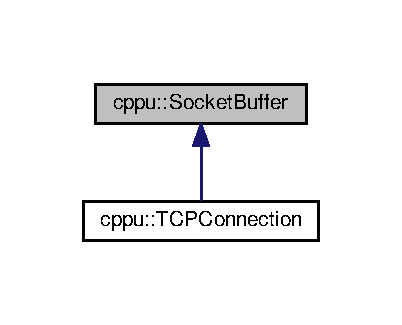
\includegraphics[width=193pt]{classcppu_1_1SocketBuffer__inherit__graph}
\end{center}
\end{figure}


Collaboration diagram for cppu\+:\+:Socket\+Buffer\+:
\nopagebreak
\begin{figure}[H]
\begin{center}
\leavevmode
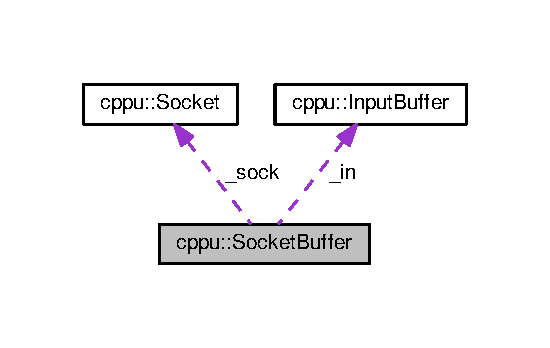
\includegraphics[width=264pt]{classcppu_1_1SocketBuffer__coll__graph}
\end{center}
\end{figure}
\subsection*{Public Member Functions}
\begin{DoxyCompactItemize}
\item 
\hypertarget{classcppu_1_1SocketBuffer_a1d6a8ae90bfcb69e6b3d2b9f97e3dc40}{}\hyperlink{classcppu_1_1SocketBuffer_a1d6a8ae90bfcb69e6b3d2b9f97e3dc40}{Socket\+Buffer} (\hyperlink{classcppu_1_1Socket}{Socket} $\ast$\hyperlink{classcppu_1_1SocketBuffer_aab887b32ee999bfdd01c9a491c04bd61}{socket}, size\+\_\+t input\+Buffer\+Size=8192, size\+\_\+t ouput\+Buffer\+Size=8192)\label{classcppu_1_1SocketBuffer_a1d6a8ae90bfcb69e6b3d2b9f97e3dc40}

\begin{DoxyCompactList}\small\item\em constructor. {\itshape socket} must be a connected T\+C\+P/\+I\+P \hyperlink{classcppu_1_1Socket}{Socket} (i.\+e. of S\+O\+C\+K\+\_\+\+S\+T\+R\+E\+A\+M type) that must {\itshape not} be deleted while the \hyperlink{classcppu_1_1SocketBuffer}{Socket\+Buffer} is used. {\itshape input\+Buffer\+Size} and {\itshape ouput\+Buffer\+Size} are the sizes of the buffers that used internally for exchanging the data. \end{DoxyCompactList}\item 
\hypertarget{classcppu_1_1SocketBuffer_ae8e387747f17f4ff3bfe036ccf11e89b}{}{\bfseries Socket\+Buffer} (\hyperlink{classcppu_1_1Socket}{Socket} \&\hyperlink{classcppu_1_1SocketBuffer_aab887b32ee999bfdd01c9a491c04bd61}{socket}, size\+\_\+t input\+Buffer\+Size=8192, size\+\_\+t ouput\+Buffer\+Size=8192)\label{classcppu_1_1SocketBuffer_ae8e387747f17f4ff3bfe036ccf11e89b}

\item 
\hypertarget{classcppu_1_1SocketBuffer_aab887b32ee999bfdd01c9a491c04bd61}{}\hyperlink{classcppu_1_1Socket}{Socket} $\ast$ \hyperlink{classcppu_1_1SocketBuffer_aab887b32ee999bfdd01c9a491c04bd61}{socket} ()\label{classcppu_1_1SocketBuffer_aab887b32ee999bfdd01c9a491c04bd61}

\begin{DoxyCompactList}\small\item\em returns the associated socket. \end{DoxyCompactList}\item 
\hypertarget{classcppu_1_1SocketBuffer_a77dfe31ad3d5660322d788daf213534e}{}int \hyperlink{classcppu_1_1SocketBuffer_a77dfe31ad3d5660322d788daf213534e}{input\+Separator} () const \label{classcppu_1_1SocketBuffer_a77dfe31ad3d5660322d788daf213534e}

\begin{DoxyCompactList}\small\item\em returns the input separator. \end{DoxyCompactList}\item 
\hypertarget{classcppu_1_1SocketBuffer_a737c72f4ce5ff73a2e7339430b6d1614}{}int \hyperlink{classcppu_1_1SocketBuffer_a737c72f4ce5ff73a2e7339430b6d1614}{output\+Separator} () const \label{classcppu_1_1SocketBuffer_a737c72f4ce5ff73a2e7339430b6d1614}

\begin{DoxyCompactList}\small\item\em returns the output separator. \end{DoxyCompactList}\item 
virtual void \hyperlink{classcppu_1_1SocketBuffer_acadf4540c1e3eba67b014753b84b482c}{set\+Input\+Separator} (int separ)
\begin{DoxyCompactList}\small\item\em changes the input separator. This function specifies the character(s) used by \hyperlink{classcppu_1_1SocketBuffer_a222769d3776b9cbd3a727ee1f0e60358}{read\+Line()} to separate successive lines\+: \end{DoxyCompactList}\item 
virtual void \hyperlink{classcppu_1_1SocketBuffer_a0e5e6a9ce3bda28b65c559c8b3c91b0f}{set\+Output\+Separator} (int separ)
\begin{DoxyCompactList}\small\item\em changes the output separator. This function specifies the character(s) used by \hyperlink{classcppu_1_1SocketBuffer_a92ae0351aaee8719d34e8c4618495d59}{write\+Line()} to separate successive lines\+: \end{DoxyCompactList}\item 
virtual ssize\+\_\+t \hyperlink{classcppu_1_1SocketBuffer_a222769d3776b9cbd3a727ee1f0e60358}{read\+Line} (std\+::string \&str)
\begin{DoxyCompactList}\small\item\em Reads a line of text from a connected socket. \hyperlink{classcppu_1_1SocketBuffer_a222769d3776b9cbd3a727ee1f0e60358}{read\+Line()} receives one line of text sent by \hyperlink{classcppu_1_1SocketBuffer_a92ae0351aaee8719d34e8c4618495d59}{write\+Line()} on the other side. The text is stored in {\itshape str}. This method blocks until the complete text line is received. \end{DoxyCompactList}\item 
virtual ssize\+\_\+t \hyperlink{classcppu_1_1SocketBuffer_a92ae0351aaee8719d34e8c4618495d59}{write\+Line} (const std\+::string \&str)
\begin{DoxyCompactList}\small\item\em Sends a line of text to a connected socket. \hyperlink{classcppu_1_1SocketBuffer_a92ae0351aaee8719d34e8c4618495d59}{write\+Line()} sends one line of text that will be received by a single call to \hyperlink{classcppu_1_1SocketBuffer_a222769d3776b9cbd3a727ee1f0e60358}{read\+Line()} on the other side (see note below). \end{DoxyCompactList}\item 
\hypertarget{classcppu_1_1SocketBuffer_a27de273ae2defbf3a5cc308310b9835e}{}virtual ssize\+\_\+t {\bfseries read} (char $\ast$buffer, size\+\_\+t len)\label{classcppu_1_1SocketBuffer_a27de273ae2defbf3a5cc308310b9835e}

\item 
\hypertarget{classcppu_1_1SocketBuffer_ab4ed032f329be2f6ecd0cba5fcd0518d}{}virtual ssize\+\_\+t {\bfseries write} (const char $\ast$str, size\+\_\+t len)\label{classcppu_1_1SocketBuffer_ab4ed032f329be2f6ecd0cba5fcd0518d}

\end{DoxyCompactItemize}
\subsection*{Protected Member Functions}
\begin{DoxyCompactItemize}
\item 
\hypertarget{classcppu_1_1SocketBuffer_ae634cbe12f6688a8d64c4579299e9802}{}virtual bool {\bfseries retrieve\+Line} (std\+::string \&str, ssize\+\_\+t received)\label{classcppu_1_1SocketBuffer_ae634cbe12f6688a8d64c4579299e9802}

\end{DoxyCompactItemize}
\subsection*{Protected Attributes}
\begin{DoxyCompactItemize}
\item 
\hypertarget{classcppu_1_1SocketBuffer_af52d0e7a5fb70ad371693c2e7f9f056b}{}size\+\_\+t {\bfseries \+\_\+in\+Size}\label{classcppu_1_1SocketBuffer_af52d0e7a5fb70ad371693c2e7f9f056b}

\item 
\hypertarget{classcppu_1_1SocketBuffer_afa2daeed2c8538030353382f48269896}{}size\+\_\+t {\bfseries \+\_\+out\+Size}\label{classcppu_1_1SocketBuffer_afa2daeed2c8538030353382f48269896}

\item 
\hypertarget{classcppu_1_1SocketBuffer_a5bf8f3a5ef56fc6f15ade71fe55b049d}{}int {\bfseries \+\_\+in\+Sep}\label{classcppu_1_1SocketBuffer_a5bf8f3a5ef56fc6f15ade71fe55b049d}

\item 
\hypertarget{classcppu_1_1SocketBuffer_a59b35cfa717476d18cc2e40c73073354}{}int {\bfseries \+\_\+out\+Sep}\label{classcppu_1_1SocketBuffer_a59b35cfa717476d18cc2e40c73073354}

\item 
\hypertarget{classcppu_1_1SocketBuffer_af60722acd94826d780bbb2477667d538}{}\hyperlink{classcppu_1_1Socket}{Socket} $\ast$ {\bfseries \+\_\+sock}\label{classcppu_1_1SocketBuffer_af60722acd94826d780bbb2477667d538}

\item 
\hypertarget{classcppu_1_1SocketBuffer_adb5986d6297496a1f92a30b1b3923072}{}struct \hyperlink{structcppu_1_1InputBuffer}{Input\+Buffer} $\ast$ {\bfseries \+\_\+in}\label{classcppu_1_1SocketBuffer_adb5986d6297496a1f92a30b1b3923072}

\end{DoxyCompactItemize}


\subsection{Detailed Description}
Preserves record boundaries when exchanging data between connected T\+C\+P/\+I\+P sockets. This class ensures that one call to \hyperlink{classcppu_1_1SocketBuffer_a92ae0351aaee8719d34e8c4618495d59}{write\+Line()} corresponds to one and exactly one call to \hyperlink{classcppu_1_1SocketBuffer_a222769d3776b9cbd3a727ee1f0e60358}{read\+Line()} on the other side. This differs from the behavior of \hyperlink{classcppu_1_1Socket_aeac77f859159715e2d63a5a0dc118788}{Socket\+::send()} and \hyperlink{classcppu_1_1Socket_a37c382af52cc02f92c0e19a0c6e0e04f}{Socket\+::receive()} because T\+C\+P/\+I\+P connected sockets do not preserve record boundaries. \hyperlink{classcppu_1_1SocketBuffer_a92ae0351aaee8719d34e8c4618495d59}{write\+Line()} and \hyperlink{classcppu_1_1SocketBuffer_a222769d3776b9cbd3a727ee1f0e60358}{read\+Line()} solve this problem by automatically adding and searching for a separator between successive lines. 

\begin{DoxySeeAlso}{See also}
\hyperlink{classcppu_1_1SocketBuffer_acadf4540c1e3eba67b014753b84b482c}{set\+Input\+Separator()} and \hyperlink{classcppu_1_1SocketBuffer_a0e5e6a9ce3bda28b65c559c8b3c91b0f}{set\+Output\+Separator()}. 
\end{DoxySeeAlso}


\subsection{Member Function Documentation}
\hypertarget{classcppu_1_1SocketBuffer_a222769d3776b9cbd3a727ee1f0e60358}{}\index{cppu\+::\+Socket\+Buffer@{cppu\+::\+Socket\+Buffer}!read\+Line@{read\+Line}}
\index{read\+Line@{read\+Line}!cppu\+::\+Socket\+Buffer@{cppu\+::\+Socket\+Buffer}}
\subsubsection[{read\+Line}]{\setlength{\rightskip}{0pt plus 5cm}ssize\+\_\+t cppu\+::\+Socket\+Buffer\+::read\+Line (
\begin{DoxyParamCaption}
\item[{std\+::string \&}]{str}
\end{DoxyParamCaption}
)\hspace{0.3cm}{\ttfamily [virtual]}}\label{classcppu_1_1SocketBuffer_a222769d3776b9cbd3a727ee1f0e60358}


Reads a line of text from a connected socket. \hyperlink{classcppu_1_1SocketBuffer_a222769d3776b9cbd3a727ee1f0e60358}{read\+Line()} receives one line of text sent by \hyperlink{classcppu_1_1SocketBuffer_a92ae0351aaee8719d34e8c4618495d59}{write\+Line()} on the other side. The text is stored in {\itshape str}. This method blocks until the complete text line is received. 

\hyperlink{classcppu_1_1SocketBuffer_a222769d3776b9cbd3a727ee1f0e60358}{read\+Line()} relies on a separator (by default, ~\newline
, ~\newline
 or ~\newline
, \begin{DoxySeeAlso}{See also}
\hyperlink{classcppu_1_1SocketBuffer_acadf4540c1e3eba67b014753b84b482c}{set\+Input\+Separator()}. This separator is automatically removed (it is not stored in {\itshape str}).
\end{DoxySeeAlso}
\begin{DoxyReturn}{Returns}
the number of bytes that were received or\+:
\begin{DoxyItemize}
\item 0\+: shutdown\+Output() was called on the other side
\item Socket\+::\+Failed (-\/1)\+: a connection error occured
\item Socket\+::\+Invalid\+Socket (-\/2)\+: the socket is invalid. The separator is counted in the value returned by \hyperlink{classcppu_1_1SocketBuffer_a222769d3776b9cbd3a727ee1f0e60358}{read\+Line()}. 
\end{DoxyItemize}
\end{DoxyReturn}
\hypertarget{classcppu_1_1SocketBuffer_acadf4540c1e3eba67b014753b84b482c}{}\index{cppu\+::\+Socket\+Buffer@{cppu\+::\+Socket\+Buffer}!set\+Input\+Separator@{set\+Input\+Separator}}
\index{set\+Input\+Separator@{set\+Input\+Separator}!cppu\+::\+Socket\+Buffer@{cppu\+::\+Socket\+Buffer}}
\subsubsection[{set\+Input\+Separator}]{\setlength{\rightskip}{0pt plus 5cm}void cppu\+::\+Socket\+Buffer\+::set\+Input\+Separator (
\begin{DoxyParamCaption}
\item[{int}]{separ}
\end{DoxyParamCaption}
)\hspace{0.3cm}{\ttfamily [virtual]}}\label{classcppu_1_1SocketBuffer_acadf4540c1e3eba67b014753b84b482c}


changes the input separator. This function specifies the character(s) used by \hyperlink{classcppu_1_1SocketBuffer_a222769d3776b9cbd3a727ee1f0e60358}{read\+Line()} to separate successive lines\+: 


\begin{DoxyItemize}
\item if {\itshape separ} $>$= 0, \hyperlink{classcppu_1_1SocketBuffer_a222769d3776b9cbd3a727ee1f0e60358}{read\+Line()} searches for {\itshape separ} to separate lines,
\item if {\itshape separ} $<$ 0, \hyperlink{classcppu_1_1SocketBuffer_a222769d3776b9cbd3a727ee1f0e60358}{read\+Line()} searches for ~\newline
,  or ~\newline
. By default, \hyperlink{classcppu_1_1SocketBuffer_a222769d3776b9cbd3a727ee1f0e60358}{read\+Line()} for ~\newline
,  or ~\newline
. \begin{DoxyNote}{Note}
If the input separator is changed, the output separator must be changed accordingly on the other side of the socket. 
\end{DoxyNote}
\begin{DoxySeeAlso}{See also}
\hyperlink{classcppu_1_1SocketBuffer_a0e5e6a9ce3bda28b65c559c8b3c91b0f}{set\+Output\+Separator()}. 
\end{DoxySeeAlso}

\end{DoxyItemize}\hypertarget{classcppu_1_1SocketBuffer_a0e5e6a9ce3bda28b65c559c8b3c91b0f}{}\index{cppu\+::\+Socket\+Buffer@{cppu\+::\+Socket\+Buffer}!set\+Output\+Separator@{set\+Output\+Separator}}
\index{set\+Output\+Separator@{set\+Output\+Separator}!cppu\+::\+Socket\+Buffer@{cppu\+::\+Socket\+Buffer}}
\subsubsection[{set\+Output\+Separator}]{\setlength{\rightskip}{0pt plus 5cm}void cppu\+::\+Socket\+Buffer\+::set\+Output\+Separator (
\begin{DoxyParamCaption}
\item[{int}]{separ}
\end{DoxyParamCaption}
)\hspace{0.3cm}{\ttfamily [virtual]}}\label{classcppu_1_1SocketBuffer_a0e5e6a9ce3bda28b65c559c8b3c91b0f}


changes the output separator. This function specifies the character(s) used by \hyperlink{classcppu_1_1SocketBuffer_a92ae0351aaee8719d34e8c4618495d59}{write\+Line()} to separate successive lines\+: 


\begin{DoxyItemize}
\item if {\itshape separ} $>$= 0, \hyperlink{classcppu_1_1SocketBuffer_a92ae0351aaee8719d34e8c4618495d59}{write\+Line()} inserts {\itshape separ} between successive lines,
\item if {\itshape separ} $<$ 0, \hyperlink{classcppu_1_1SocketBuffer_a92ae0351aaee8719d34e8c4618495d59}{write\+Line()} inserts ~\newline
 between successive lines. By default, \hyperlink{classcppu_1_1SocketBuffer_a92ae0351aaee8719d34e8c4618495d59}{write\+Line()} inserts ~\newline
. \begin{DoxyNote}{Note}
If the output separator is changed, the input separator must be changed accordingly on the other side of the socket. 
\end{DoxyNote}
\begin{DoxySeeAlso}{See also}
\hyperlink{classcppu_1_1SocketBuffer_acadf4540c1e3eba67b014753b84b482c}{set\+Input\+Separator()}. 
\end{DoxySeeAlso}

\end{DoxyItemize}\hypertarget{classcppu_1_1SocketBuffer_a92ae0351aaee8719d34e8c4618495d59}{}\index{cppu\+::\+Socket\+Buffer@{cppu\+::\+Socket\+Buffer}!write\+Line@{write\+Line}}
\index{write\+Line@{write\+Line}!cppu\+::\+Socket\+Buffer@{cppu\+::\+Socket\+Buffer}}
\subsubsection[{write\+Line}]{\setlength{\rightskip}{0pt plus 5cm}ssize\+\_\+t cppu\+::\+Socket\+Buffer\+::write\+Line (
\begin{DoxyParamCaption}
\item[{const std\+::string \&}]{str}
\end{DoxyParamCaption}
)\hspace{0.3cm}{\ttfamily [virtual]}}\label{classcppu_1_1SocketBuffer_a92ae0351aaee8719d34e8c4618495d59}


Sends a line of text to a connected socket. \hyperlink{classcppu_1_1SocketBuffer_a92ae0351aaee8719d34e8c4618495d59}{write\+Line()} sends one line of text that will be received by a single call to \hyperlink{classcppu_1_1SocketBuffer_a222769d3776b9cbd3a727ee1f0e60358}{read\+Line()} on the other side (see note below). 

\hyperlink{classcppu_1_1SocketBuffer_a92ae0351aaee8719d34e8c4618495d59}{write\+Line()} relies on a separator (~\newline
 by default, \begin{DoxySeeAlso}{See also}
\hyperlink{classcppu_1_1SocketBuffer_a0e5e6a9ce3bda28b65c559c8b3c91b0f}{set\+Output\+Separator()}) that is automatically inserted between successive lines ().
\end{DoxySeeAlso}
\begin{DoxyReturn}{Returns}
the number of bytes that were sent or\+:
\begin{DoxyItemize}
\item 0\+: shutdown\+Input() was called on the other side
\item Socket\+::\+Failed (-\/1)\+: a connection error occured
\item Socket\+::\+Invalid\+Socket (-\/2)\+: the socket is invalid. The separator is counted in the value returned by \hyperlink{classcppu_1_1SocketBuffer_a92ae0351aaee8719d34e8c4618495d59}{write\+Line()}.
\end{DoxyItemize}
\end{DoxyReturn}
\begin{DoxyNote}{Note}
if {\itshape str} constains occurences of the separator, \hyperlink{classcppu_1_1SocketBuffer_a222769d3776b9cbd3a727ee1f0e60358}{read\+Line()} will be called several times on the other side. 
\end{DoxyNote}


The documentation for this class was generated from the following files\+:\begin{DoxyCompactItemize}
\item 
cpp\+Socket.\+h\item 
cpp\+Socket.\+cpp\end{DoxyCompactItemize}

\hypertarget{classcppu_1_1TCPConnection}{}\section{cppu\+:\+:T\+C\+P\+Connection Class Reference}
\label{classcppu_1_1TCPConnection}\index{cppu\+::\+T\+C\+P\+Connection@{cppu\+::\+T\+C\+P\+Connection}}


Connection with a given client. Each \hyperlink{classcppu_1_1TCPConnection}{T\+C\+P\+Connection} uses a different thread.  




{\ttfamily \#include $<$tcp\+Server.\+h$>$}



Inheritance diagram for cppu\+:\+:T\+C\+P\+Connection\+:
\nopagebreak
\begin{figure}[H]
\begin{center}
\leavevmode
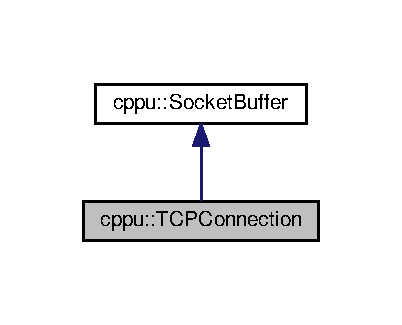
\includegraphics[width=193pt]{classcppu_1_1TCPConnection__inherit__graph}
\end{center}
\end{figure}


Collaboration diagram for cppu\+:\+:T\+C\+P\+Connection\+:
\nopagebreak
\begin{figure}[H]
\begin{center}
\leavevmode
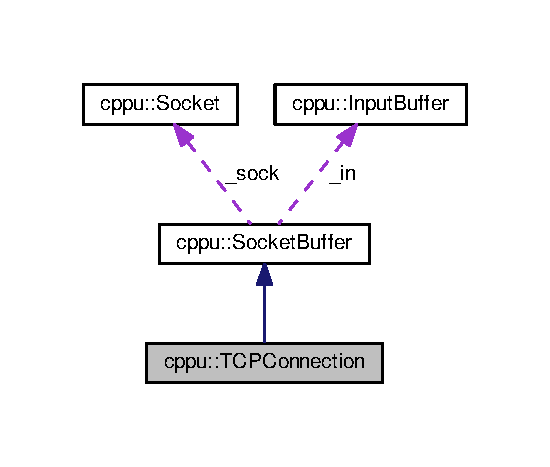
\includegraphics[width=264pt]{classcppu_1_1TCPConnection__coll__graph}
\end{center}
\end{figure}
\subsection*{Public Member Functions}
\begin{DoxyCompactItemize}
\item 
\hypertarget{classcppu_1_1TCPConnection_a4186946c7c22e3c2cebe3a97aa78f5f7}{}\hyperlink{classcppu_1_1TCPServer}{T\+C\+P\+Server} \& {\bfseries server} ()\label{classcppu_1_1TCPConnection_a4186946c7c22e3c2cebe3a97aa78f5f7}

\item 
\hypertarget{classcppu_1_1TCPConnection_a4663875b80fced790502880c72e6e672}{}pthread\+\_\+t {\bfseries thread} ()\label{classcppu_1_1TCPConnection_a4663875b80fced790502880c72e6e672}

\end{DoxyCompactItemize}
\subsection*{Friends}
\begin{DoxyCompactItemize}
\item 
\hypertarget{classcppu_1_1TCPConnection_ae4cfdb1814d91a8d28dadb49adda68f0}{}class {\bfseries T\+C\+P\+Server}\label{classcppu_1_1TCPConnection_ae4cfdb1814d91a8d28dadb49adda68f0}

\end{DoxyCompactItemize}
\subsection*{Additional Inherited Members}


\subsection{Detailed Description}
Connection with a given client. Each \hyperlink{classcppu_1_1TCPConnection}{T\+C\+P\+Connection} uses a different thread. 

The documentation for this class was generated from the following files\+:\begin{DoxyCompactItemize}
\item 
tcp\+Server.\+h\item 
tcp\+Server.\+cpp\end{DoxyCompactItemize}

\hypertarget{classcppu_1_1TCPLock}{}\section{cppu\+:\+:T\+C\+P\+Lock Class Reference}
\label{classcppu_1_1TCPLock}\index{cppu\+::\+T\+C\+P\+Lock@{cppu\+::\+T\+C\+P\+Lock}}


Locks the server in read mode or in write mode. Must be created {\itshape in the stack} by the callback method.  




{\ttfamily \#include $<$tcp\+Server.\+h$>$}

\subsection*{Public Member Functions}
\begin{DoxyCompactItemize}
\item 
\hyperlink{classcppu_1_1TCPLock_ad9ff8205f334918a69746ef90f731877}{T\+C\+P\+Lock} (\hyperlink{classcppu_1_1TCPConnection}{T\+C\+P\+Connection} \&cnx, bool write\+Mode=false)
\begin{DoxyCompactList}\small\item\em locks the server in {\itshape write} or {\itshape read} mode. In order to avoid concurrency problems between threads, the callback method ( \end{DoxyCompactList}\end{DoxyCompactItemize}


\subsection{Detailed Description}
Locks the server in read mode or in write mode. Must be created {\itshape in the stack} by the callback method. 

\subsection{Constructor \& Destructor Documentation}
\hypertarget{classcppu_1_1TCPLock_ad9ff8205f334918a69746ef90f731877}{}\index{cppu\+::\+T\+C\+P\+Lock@{cppu\+::\+T\+C\+P\+Lock}!T\+C\+P\+Lock@{T\+C\+P\+Lock}}
\index{T\+C\+P\+Lock@{T\+C\+P\+Lock}!cppu\+::\+T\+C\+P\+Lock@{cppu\+::\+T\+C\+P\+Lock}}
\subsubsection[{T\+C\+P\+Lock}]{\setlength{\rightskip}{0pt plus 5cm}cppu\+::\+T\+C\+P\+Lock\+::\+T\+C\+P\+Lock (
\begin{DoxyParamCaption}
\item[{{\bf T\+C\+P\+Connection} \&}]{cnx, }
\item[{bool}]{write\+Mode = {\ttfamily false}}
\end{DoxyParamCaption}
)}\label{classcppu_1_1TCPLock_ad9ff8205f334918a69746ef90f731877}


locks the server in {\itshape write} or {\itshape read} mode. In order to avoid concurrency problems between threads, the callback method ( 

\begin{DoxySeeAlso}{See also}
set\+Callback()) can create a \hyperlink{classcppu_1_1TCPLock}{T\+C\+P\+Lock} object {\itshape in the stack} before performing a computation.
\end{DoxySeeAlso}
{\itshape write\+Mode} must be true if the callback changes data and false (the default) otherwise. A write\+Mode lock blocks all other locks (and the corresponding threads) until the callback method returns. 

The documentation for this class was generated from the following files\+:\begin{DoxyCompactItemize}
\item 
tcp\+Server.\+h\item 
tcp\+Server.\+cpp\end{DoxyCompactItemize}

\hypertarget{classcppu_1_1TCPServer}{}\section{cppu\+:\+:T\+C\+P\+Server Class Reference}
\label{classcppu_1_1TCPServer}\index{cppu\+::\+T\+C\+P\+Server@{cppu\+::\+T\+C\+P\+Server}}


T\+C\+P/\+I\+P I\+Pv4 server. The server supports T\+C\+P/\+I\+P A\+F\+\_\+\+I\+N\+E\+T connections (following the I\+Pv4 Internet protocol) with multiple clients. One thread is used per client.  




{\ttfamily \#include $<$tcp\+Server.\+h$>$}



Collaboration diagram for cppu\+:\+:T\+C\+P\+Server\+:
\nopagebreak
\begin{figure}[H]
\begin{center}
\leavevmode
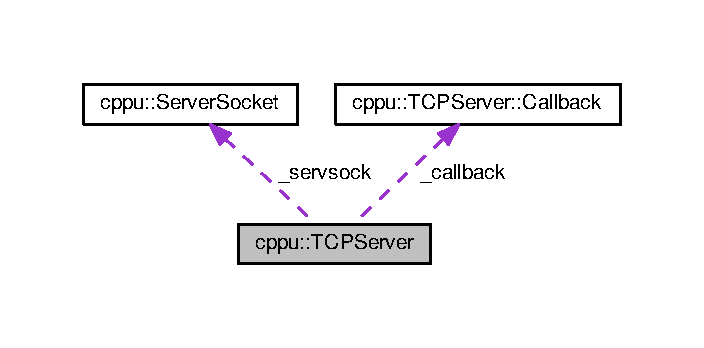
\includegraphics[width=338pt]{classcppu_1_1TCPServer__coll__graph}
\end{center}
\end{figure}
\subsection*{Classes}
\begin{DoxyCompactItemize}
\item 
struct \hyperlink{structcppu_1_1TCPServer_1_1Callback}{Callback}
\begin{DoxyCompactList}\small\item\em \hyperlink{structcppu_1_1TCPServer_1_1Callback}{Callback} interface. \end{DoxyCompactList}\item 
struct \hyperlink{structcppu_1_1TCPServer_1_1CallbackMethod}{Callback\+Method}
\end{DoxyCompactItemize}
\subsection*{Public Member Functions}
\begin{DoxyCompactItemize}
\item 
\hypertarget{classcppu_1_1TCPServer_a48074f8409f580f6cf7b0be80200f9f3}{}\hyperlink{classcppu_1_1TCPServer_a48074f8409f580f6cf7b0be80200f9f3}{T\+C\+P\+Server} ()\label{classcppu_1_1TCPServer_a48074f8409f580f6cf7b0be80200f9f3}

\begin{DoxyCompactList}\small\item\em constructor\+: initializes the \hyperlink{classcppu_1_1TCPServer}{T\+C\+P\+Server}. \end{DoxyCompactList}\item 
\hypertarget{classcppu_1_1TCPServer_ababd20111e0cf4e14396433e56ca086e}{}virtual \hyperlink{classcppu_1_1TCPServer_ababd20111e0cf4e14396433e56ca086e}{$\sim$\+T\+C\+P\+Server} ()\label{classcppu_1_1TCPServer_ababd20111e0cf4e14396433e56ca086e}

\begin{DoxyCompactList}\small\item\em destructor\+: cleans up the \hyperlink{classcppu_1_1TCPServer}{T\+C\+P\+Server}. \end{DoxyCompactList}\item 
virtual int \hyperlink{classcppu_1_1TCPServer_a98e00d62745812b17bdee9f07f2070c4}{run} (int port)
\begin{DoxyCompactList}\small\item\em starts the \hyperlink{classcppu_1_1TCPServer}{T\+C\+P\+Server}. \hyperlink{classcppu_1_1TCPServer_a98e00d62745812b17bdee9f07f2070c4}{run()} binds an internal \hyperlink{classcppu_1_1ServerSocket}{Server\+Socket} to {\itshape port} then starts an infinite loop that processes connection requests from clients. \end{DoxyCompactList}\item 
{\footnotesize template$<$class T $>$ }\\void \hyperlink{classcppu_1_1TCPServer_a7d4fdb93439015934004755fde72945b}{set\+Callback} (T \&object, bool(T\+::$\ast$method)(\hyperlink{classcppu_1_1TCPConnection}{T\+C\+P\+Connection} \&cnx, const std\+::string \&request, std\+::string \&response))
\begin{DoxyCompactList}\small\item\em changes the callback method of the \hyperlink{classcppu_1_1TCPServer}{T\+C\+P\+Server}. This callback is called each time the \hyperlink{classcppu_1_1TCPServer}{T\+C\+P\+Server} receives a request from a client. It can be any method of {\itshape object} with the following parameters\+: \end{DoxyCompactList}\item 
void \hyperlink{classcppu_1_1TCPServer_a94d3d97b03d5e3e48609e405d8dd7897}{set\+Callback} (\hyperlink{structcppu_1_1TCPServer_1_1Callback}{Callback} \&callback)
\begin{DoxyCompactList}\small\item\em changes the callback object of the \hyperlink{classcppu_1_1TCPServer}{T\+C\+P\+Server}. \end{DoxyCompactList}\item 
\hypertarget{classcppu_1_1TCPServer_a6428b63a4440045050dba4f33bb454bf}{}\hyperlink{classcppu_1_1ServerSocket}{Server\+Socket} \& \hyperlink{classcppu_1_1TCPServer_a6428b63a4440045050dba4f33bb454bf}{server\+Socket} ()\label{classcppu_1_1TCPServer_a6428b63a4440045050dba4f33bb454bf}

\begin{DoxyCompactList}\small\item\em returns the internal \hyperlink{classcppu_1_1ServerSocket}{Server\+Socket}. \end{DoxyCompactList}\item 
\hypertarget{classcppu_1_1TCPServer_afc47ca4476d9c75d5ea88f73e2acd6d5}{}virtual void \hyperlink{classcppu_1_1TCPServer_afc47ca4476d9c75d5ea88f73e2acd6d5}{error} (const std\+::string \&msg, const \hyperlink{classcppu_1_1TCPConnection}{T\+C\+P\+Connection} $\ast$=nullptr)\label{classcppu_1_1TCPServer_afc47ca4476d9c75d5ea88f73e2acd6d5}

\begin{DoxyCompactList}\small\item\em prints warning and error messages on the terminal. \end{DoxyCompactList}\end{DoxyCompactItemize}
\subsection*{Protected Member Functions}
\begin{DoxyCompactItemize}
\item 
\hypertarget{classcppu_1_1TCPServer_abe314b95a31c88b479c81ec9bf123c65}{}virtual \hyperlink{classcppu_1_1TCPConnection}{T\+C\+P\+Connection} $\ast$ \hyperlink{classcppu_1_1TCPServer_abe314b95a31c88b479c81ec9bf123c65}{create\+Cnx} (\hyperlink{classcppu_1_1Socket}{Socket} $\ast$)\label{classcppu_1_1TCPServer_abe314b95a31c88b479c81ec9bf123c65}

\begin{DoxyCompactList}\small\item\em creates a new connection that starts a new thread for listening this socket. \end{DoxyCompactList}\end{DoxyCompactItemize}
\subsection*{Protected Attributes}
\begin{DoxyCompactItemize}
\item 
\hypertarget{classcppu_1_1TCPServer_a8e4422abf23dc5bd195d05a3e9eee167}{}\hyperlink{classcppu_1_1ServerSocket}{Server\+Socket} {\bfseries \+\_\+servsock}\label{classcppu_1_1TCPServer_a8e4422abf23dc5bd195d05a3e9eee167}

\item 
\hypertarget{classcppu_1_1TCPServer_abe36d427d7b047cdd342e282611c841e}{}std\+::shared\+\_\+ptr$<$ \hyperlink{structcppu_1_1TCPServer_1_1Callback}{Callback} $>$ {\bfseries \+\_\+callback\+Ptr}\label{classcppu_1_1TCPServer_abe36d427d7b047cdd342e282611c841e}

\item 
\hypertarget{classcppu_1_1TCPServer_a68940bd70ac6941ca49d1e51b631f5e9}{}\hyperlink{structcppu_1_1TCPServer_1_1Callback}{Callback} $\ast$ {\bfseries \+\_\+callback}\label{classcppu_1_1TCPServer_a68940bd70ac6941ca49d1e51b631f5e9}

\item 
\hypertarget{classcppu_1_1TCPServer_aea2dbb4b5762044217096e52cd559b97}{}pthread\+\_\+rwlock\+\_\+t {\bfseries \+\_\+threadlock}\label{classcppu_1_1TCPServer_aea2dbb4b5762044217096e52cd559b97}

\end{DoxyCompactItemize}
\subsection*{Friends}
\begin{DoxyCompactItemize}
\item 
\hypertarget{classcppu_1_1TCPServer_a94abdeb80587f39a869fde6f24522a78}{}class {\bfseries T\+C\+P\+Lock}\label{classcppu_1_1TCPServer_a94abdeb80587f39a869fde6f24522a78}

\item 
\hypertarget{classcppu_1_1TCPServer_a9d1c27bdfcdd48c5f07a5d0dce43b346}{}class {\bfseries T\+C\+P\+Connection}\label{classcppu_1_1TCPServer_a9d1c27bdfcdd48c5f07a5d0dce43b346}

\end{DoxyCompactItemize}


\subsection{Detailed Description}
T\+C\+P/\+I\+P I\+Pv4 server. The server supports T\+C\+P/\+I\+P A\+F\+\_\+\+I\+N\+E\+T connections (following the I\+Pv4 Internet protocol) with multiple clients. One thread is used per client. 

Call \hyperlink{classcppu_1_1TCPServer_a7d4fdb93439015934004755fde72945b}{set\+Callback()} to specify the callback method that will be invoked each time a request is sent by a client then \hyperlink{classcppu_1_1TCPServer_a98e00d62745812b17bdee9f07f2070c4}{run()} to start the server.

Requests can be processed concurrently thanks to threads. To avoid concurrency problems the callback can perform a read or write lock (\begin{DoxySeeAlso}{See also}
\hyperlink{classcppu_1_1TCPLock}{T\+C\+P\+Lock}). 
\end{DoxySeeAlso}


\subsection{Member Function Documentation}
\hypertarget{classcppu_1_1TCPServer_a98e00d62745812b17bdee9f07f2070c4}{}\index{cppu\+::\+T\+C\+P\+Server@{cppu\+::\+T\+C\+P\+Server}!run@{run}}
\index{run@{run}!cppu\+::\+T\+C\+P\+Server@{cppu\+::\+T\+C\+P\+Server}}
\subsubsection[{run}]{\setlength{\rightskip}{0pt plus 5cm}int cppu\+::\+T\+C\+P\+Server\+::run (
\begin{DoxyParamCaption}
\item[{int}]{port}
\end{DoxyParamCaption}
)\hspace{0.3cm}{\ttfamily [virtual]}}\label{classcppu_1_1TCPServer_a98e00d62745812b17bdee9f07f2070c4}


starts the \hyperlink{classcppu_1_1TCPServer}{T\+C\+P\+Server}. \hyperlink{classcppu_1_1TCPServer_a98e00d62745812b17bdee9f07f2070c4}{run()} binds an internal \hyperlink{classcppu_1_1ServerSocket}{Server\+Socket} to {\itshape port} then starts an infinite loop that processes connection requests from clients. 

For each successful connection request, a \hyperlink{classcppu_1_1TCPConnection}{T\+C\+P\+Connection} object is created. This object starts a thread that processes incoming requests from its client. A callback method (\begin{DoxySeeAlso}{See also}
\hyperlink{classcppu_1_1TCPServer_a7d4fdb93439015934004755fde72945b}{set\+Callback()}) is invoked for each request.
\end{DoxySeeAlso}
\begin{DoxyReturn}{Returns}
0 on normal termination or a negative value if the \hyperlink{classcppu_1_1ServerSocket}{Server\+Socket} could not be bound (value is then one of \hyperlink{classcppu_1_1Socket_a49ea5cb079bd7ae97ecf7eb30c9d9e5f}{Socket\+::\+Errors}). 
\end{DoxyReturn}
\hypertarget{classcppu_1_1TCPServer_a7d4fdb93439015934004755fde72945b}{}\index{cppu\+::\+T\+C\+P\+Server@{cppu\+::\+T\+C\+P\+Server}!set\+Callback@{set\+Callback}}
\index{set\+Callback@{set\+Callback}!cppu\+::\+T\+C\+P\+Server@{cppu\+::\+T\+C\+P\+Server}}
\subsubsection[{set\+Callback}]{\setlength{\rightskip}{0pt plus 5cm}template$<$class T $>$ void cppu\+::\+T\+C\+P\+Server\+::set\+Callback (
\begin{DoxyParamCaption}
\item[{T \&}]{object, }
\item[{bool(T\+::$\ast$)({\bf T\+C\+P\+Connection} \&cnx, const std\+::string \&request, std\+::string \&response)}]{method}
\end{DoxyParamCaption}
)\hspace{0.3cm}{\ttfamily [inline]}}\label{classcppu_1_1TCPServer_a7d4fdb93439015934004755fde72945b}


changes the callback method of the \hyperlink{classcppu_1_1TCPServer}{T\+C\+P\+Server}. This callback is called each time the \hyperlink{classcppu_1_1TCPServer}{T\+C\+P\+Server} receives a request from a client. It can be any method of {\itshape object} with the following parameters\+: 


\begin{DoxyItemize}
\item {\itshape cnx} is the connection with the client sending the request
\item {\itshape request} contains the data sent by the client
\item {\itshape response} will be sent to the client as a response The connection is closed if the callback returns false.
\end{DoxyItemize}

To avoid concurrency problems, the callback should perform a read or write lock (\begin{DoxySeeAlso}{See also}
\hyperlink{classcppu_1_1TCPLock}{T\+C\+P\+Lock}) before performing a computation. 
\end{DoxySeeAlso}
\hypertarget{classcppu_1_1TCPServer_a94d3d97b03d5e3e48609e405d8dd7897}{}\index{cppu\+::\+T\+C\+P\+Server@{cppu\+::\+T\+C\+P\+Server}!set\+Callback@{set\+Callback}}
\index{set\+Callback@{set\+Callback}!cppu\+::\+T\+C\+P\+Server@{cppu\+::\+T\+C\+P\+Server}}
\subsubsection[{set\+Callback}]{\setlength{\rightskip}{0pt plus 5cm}void cppu\+::\+T\+C\+P\+Server\+::set\+Callback (
\begin{DoxyParamCaption}
\item[{{\bf Callback} \&}]{callback}
\end{DoxyParamCaption}
)\hspace{0.3cm}{\ttfamily [inline]}}\label{classcppu_1_1TCPServer_a94d3d97b03d5e3e48609e405d8dd7897}


changes the callback object of the \hyperlink{classcppu_1_1TCPServer}{T\+C\+P\+Server}. 

\begin{DoxySeeAlso}{See also}
set\+Callback(object, method). 
\end{DoxySeeAlso}


The documentation for this class was generated from the following files\+:\begin{DoxyCompactItemize}
\item 
tcp\+Server.\+h\item 
tcp\+Server.\+cpp\end{DoxyCompactItemize}

\hypertarget{classVideo}{}\section{Video Class Reference}
\label{classVideo}\index{Video@{Video}}


\hyperlink{classVideo}{Video} class, extends the abstract class \hyperlink{classMultimediaObject}{Multimedia\+Object}.  




{\ttfamily \#include $<$Video.\+h$>$}



Inheritance diagram for Video\+:
\nopagebreak
\begin{figure}[H]
\begin{center}
\leavevmode
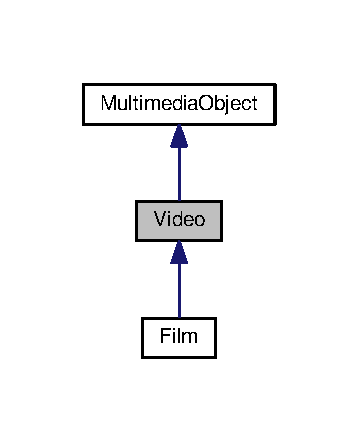
\includegraphics[width=172pt]{classVideo__inherit__graph}
\end{center}
\end{figure}


Collaboration diagram for Video\+:
\nopagebreak
\begin{figure}[H]
\begin{center}
\leavevmode
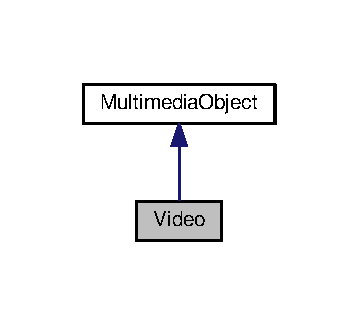
\includegraphics[width=172pt]{classVideo__coll__graph}
\end{center}
\end{figure}
\subsection*{Public Member Functions}
\begin{DoxyCompactItemize}
\item 
virtual \hyperlink{classVideo_a9a4f47fd7672b90c86d4c10176f89bb3}{$\sim$\+Video} ()
\begin{DoxyCompactList}\small\item\em Destroys the object. \end{DoxyCompactList}\item 
\hypertarget{classVideo_ac973e3d02151bb2bf7b75deda0c2ca5a}{}\hyperlink{classVideo_ac973e3d02151bb2bf7b75deda0c2ca5a}{Video} ()\label{classVideo_ac973e3d02151bb2bf7b75deda0c2ca5a}

\begin{DoxyCompactList}\small\item\em Creates the object. \end{DoxyCompactList}\item 
\hyperlink{classVideo_a0e70b25d96356f5ea3413f8f56cef897}{Video} (const string \&name, const string \&pathname, const int \&\+\_\+length)
\begin{DoxyCompactList}\small\item\em Creates the object. \end{DoxyCompactList}\item 
int \hyperlink{classVideo_afb9ed2097e0367a3c417321115ab965b}{get\+Length} () const 
\begin{DoxyCompactList}\small\item\em Gets the length. \end{DoxyCompactList}\item 
string \hyperlink{classVideo_a675d26365c71c29bc4b4b50ec2b36bc6}{get\+Class\+Name} () const override
\begin{DoxyCompactList}\small\item\em Gets the class name. \end{DoxyCompactList}\item 
void \hyperlink{classVideo_a90609ca4de9b4465e5facc27cc4b08e2}{set\+Length} (const int \&\+\_\+length)
\begin{DoxyCompactList}\small\item\em Sets the length. \end{DoxyCompactList}\item 
void \hyperlink{classVideo_a8acaac2f61e1989cf3a7dcafd14d8daf}{display} (ostream \&os) const override
\begin{DoxyCompactList}\small\item\em Displays info on the video. \end{DoxyCompactList}\item 
\hypertarget{classVideo_a61a4f3672781ab2db2d79dbbb2b1c228}{}void \hyperlink{classVideo_a61a4f3672781ab2db2d79dbbb2b1c228}{play} () const override\label{classVideo_a61a4f3672781ab2db2d79dbbb2b1c228}

\begin{DoxyCompactList}\small\item\em Plays the video using mpv. \end{DoxyCompactList}\item 
void \hyperlink{classVideo_ae71c8af72630d7d145bd948121aac01b}{write} (ostream \&os) const override
\begin{DoxyCompactList}\small\item\em Used to write the video\textquotesingle{}s content, in a file for instance. \end{DoxyCompactList}\item 
void \hyperlink{classVideo_a82ebc9192a50d9235f733a50f6710951}{read} (istream \&is) override
\begin{DoxyCompactList}\small\item\em Used to read the video\textquotesingle{}s content, from a file for instance. \end{DoxyCompactList}\end{DoxyCompactItemize}


\subsection{Detailed Description}
\hyperlink{classVideo}{Video} class, extends the abstract class \hyperlink{classMultimediaObject}{Multimedia\+Object}. 

\subsection{Constructor \& Destructor Documentation}
\hypertarget{classVideo_a9a4f47fd7672b90c86d4c10176f89bb3}{}\index{Video@{Video}!````~Video@{$\sim$\+Video}}
\index{````~Video@{$\sim$\+Video}!Video@{Video}}
\subsubsection[{$\sim$\+Video}]{\setlength{\rightskip}{0pt plus 5cm}vid\+::$\sim$\+Video (
\begin{DoxyParamCaption}
{}
\end{DoxyParamCaption}
)\hspace{0.3cm}{\ttfamily [virtual]}}\label{classVideo_a9a4f47fd7672b90c86d4c10176f89bb3}


Destroys the object. 

Destructor used just to keep track of the objects. \hypertarget{classVideo_a0e70b25d96356f5ea3413f8f56cef897}{}\index{Video@{Video}!Video@{Video}}
\index{Video@{Video}!Video@{Video}}
\subsubsection[{Video}]{\setlength{\rightskip}{0pt plus 5cm}vid\+::\+Video (
\begin{DoxyParamCaption}
\item[{const string \&}]{name, }
\item[{const string \&}]{pathname, }
\item[{const int \&}]{\+\_\+length}
\end{DoxyParamCaption}
)}\label{classVideo_a0e70b25d96356f5ea3413f8f56cef897}


Creates the object. 


\begin{DoxyParams}[1]{Parameters}
\mbox{\tt in}  & {\em name} & The name \\
\hline
\mbox{\tt in}  & {\em pathname} & The pathname \\
\hline
\mbox{\tt in}  & {\em \+\_\+length} & The length \\
\hline
\end{DoxyParams}


\subsection{Member Function Documentation}
\hypertarget{classVideo_a8acaac2f61e1989cf3a7dcafd14d8daf}{}\index{Video@{Video}!display@{display}}
\index{display@{display}!Video@{Video}}
\subsubsection[{display}]{\setlength{\rightskip}{0pt plus 5cm}void vid\+::display (
\begin{DoxyParamCaption}
\item[{ostream \&}]{os}
\end{DoxyParamCaption}
) const\hspace{0.3cm}{\ttfamily [override]}, {\ttfamily [virtual]}}\label{classVideo_a8acaac2f61e1989cf3a7dcafd14d8daf}


Displays info on the video. 


\begin{DoxyParams}{Parameters}
{\em os} & The output stream. \\
\hline
\end{DoxyParams}


Reimplemented from \hyperlink{classMultimediaObject_a9249406bc68f3aea92c87744c3f657da}{Multimedia\+Object}.

\hypertarget{classVideo_a675d26365c71c29bc4b4b50ec2b36bc6}{}\index{Video@{Video}!get\+Class\+Name@{get\+Class\+Name}}
\index{get\+Class\+Name@{get\+Class\+Name}!Video@{Video}}
\subsubsection[{get\+Class\+Name}]{\setlength{\rightskip}{0pt plus 5cm}string vid\+::get\+Class\+Name (
\begin{DoxyParamCaption}
{}
\end{DoxyParamCaption}
) const\hspace{0.3cm}{\ttfamily [override]}, {\ttfamily [virtual]}}\label{classVideo_a675d26365c71c29bc4b4b50ec2b36bc6}


Gets the class name. 

\begin{DoxyReturn}{Returns}
The class name. 
\end{DoxyReturn}


Reimplemented from \hyperlink{classMultimediaObject_a9eca3c9328fe9141dbdfd571e348aded}{Multimedia\+Object}.

\hypertarget{classVideo_afb9ed2097e0367a3c417321115ab965b}{}\index{Video@{Video}!get\+Length@{get\+Length}}
\index{get\+Length@{get\+Length}!Video@{Video}}
\subsubsection[{get\+Length}]{\setlength{\rightskip}{0pt plus 5cm}int vid\+::get\+Length (
\begin{DoxyParamCaption}
{}
\end{DoxyParamCaption}
) const}\label{classVideo_afb9ed2097e0367a3c417321115ab965b}


Gets the length. 

\begin{DoxyReturn}{Returns}
The length. 
\end{DoxyReturn}
\hypertarget{classVideo_a82ebc9192a50d9235f733a50f6710951}{}\index{Video@{Video}!read@{read}}
\index{read@{read}!Video@{Video}}
\subsubsection[{read}]{\setlength{\rightskip}{0pt plus 5cm}void vid\+::read (
\begin{DoxyParamCaption}
\item[{istream \&}]{is}
\end{DoxyParamCaption}
)\hspace{0.3cm}{\ttfamily [override]}, {\ttfamily [virtual]}}\label{classVideo_a82ebc9192a50d9235f733a50f6710951}


Used to read the video\textquotesingle{}s content, from a file for instance. 


\begin{DoxyParams}{Parameters}
{\em is} & The input stream. \\
\hline
\end{DoxyParams}


Reimplemented from \hyperlink{classMultimediaObject_af8689299cabe973f9828a69b84ebbce7}{Multimedia\+Object}.

\hypertarget{classVideo_a90609ca4de9b4465e5facc27cc4b08e2}{}\index{Video@{Video}!set\+Length@{set\+Length}}
\index{set\+Length@{set\+Length}!Video@{Video}}
\subsubsection[{set\+Length}]{\setlength{\rightskip}{0pt plus 5cm}void vid\+::set\+Length (
\begin{DoxyParamCaption}
\item[{const int \&}]{\+\_\+length}
\end{DoxyParamCaption}
)}\label{classVideo_a90609ca4de9b4465e5facc27cc4b08e2}


Sets the length. 


\begin{DoxyParams}[1]{Parameters}
\mbox{\tt in}  & {\em \+\_\+length} & The length \\
\hline
\end{DoxyParams}
\hypertarget{classVideo_ae71c8af72630d7d145bd948121aac01b}{}\index{Video@{Video}!write@{write}}
\index{write@{write}!Video@{Video}}
\subsubsection[{write}]{\setlength{\rightskip}{0pt plus 5cm}void vid\+::write (
\begin{DoxyParamCaption}
\item[{ostream \&}]{os}
\end{DoxyParamCaption}
) const\hspace{0.3cm}{\ttfamily [override]}, {\ttfamily [virtual]}}\label{classVideo_ae71c8af72630d7d145bd948121aac01b}


Used to write the video\textquotesingle{}s content, in a file for instance. 


\begin{DoxyParams}{Parameters}
{\em os} & The output stream. \\
\hline
\end{DoxyParams}


Reimplemented from \hyperlink{classMultimediaObject_af838c533bbfc85230c8569dd16be457b}{Multimedia\+Object}.



The documentation for this class was generated from the following files\+:\begin{DoxyCompactItemize}
\item 
Video.\+h\item 
Video.\+cpp\end{DoxyCompactItemize}

%--- End generated contents ---

% Index
\backmatter
\newpage
\phantomsection
\clearemptydoublepage
\addcontentsline{toc}{chapter}{Index}
\printindex

\end{document}
